\documentclass[preprint,12pt]{elsarticle}

\usepackage{amsmath,amssymb}
\usepackage{booktabs}
\usepackage{tabularx}
\usepackage{threeparttable}
\usepackage{array}
\usepackage{graphicx}
\usepackage{xcolor}
\usepackage{microtype}
\usepackage{url}
\usepackage{enumitem}
\usepackage{multirow}
\usepackage{makecell}
\usepackage{adjustbox}
\usepackage{pdflscape}
\usepackage{longtable}
\usepackage{eso-pic}
\usepackage{etoolbox}
\usepackage{float}

\journal{Applied Energy}
\biboptions{sort&compress}

\newcolumntype{Y}{>{\raggedright\arraybackslash}X}
\newcolumntype{P}[1]{>{\raggedright\arraybackslash}p{#1}}
\newcommand{\coo}{CO$_2$}
\newcommand{\qdecem}{Q-DECEM}
\newcommand{\wmase}{WMASE}
\newcommand{\figpanel}[3]{%
  \begin{minipage}[t]{#1}
    \centering
    \textbf{(#2)}\\[-0.5ex]
    \includegraphics[width=\linewidth]{#3}
  \end{minipage}}
\newcommand{\landscapepagenumber}{%
  \AtPageUpperLeft{%
    \put(\LenToUnit{\dimexpr\paperwidth-12mm\relax},\LenToUnit{-.5\paperheight}){%
      \makebox(0,0){\rotatebox{90}{\thepage}}}}}
\AtBeginEnvironment{table}{\footnotesize}
\AtBeginEnvironment{table*}{\footnotesize}
\begin{document}
\begin{frontmatter}

\title{Q-DECEM: Electricity-Grid Carbon-Intensity Dynamics as a Joint Predictive Signal for Quarterly UK CO$_2$ Emissions: A Decision-Oriented, Multi-Horizon Forecasting Framework}

\author[1]{Mohsen Asghari Ilani\corref{cor1}}
\ead{2238065@swansea.ac.uk}
\ead[url]{https://orcid.org/0000-0003-0189-6956}

\author[2]{Hamidreza Eskandari\corref{cor1}}
\ead{hamidreza.eskandari@swansea.ac.uk}
\ead[url]{https://orcid.org/0000-0002-5515-9399}


\author[3]{Mike Banad\corref{cor1}}
\ead{bana@ou.edu}
\ead[url]{https://orcid.org/0000-0002-4667-6650}


\affiliation[1]{organization={School of Management, Swansea University},
  city={Swansea},
  postcode={SA1 8EN},
  state={Wales},
  country={United Kingdom}}
\cortext[cor1]{Corresponding author.}





\affiliation[3]{organization={School of Electrical and Computer Engineering},
  addressline={University of Oklahoma},
  city={Norman},
  country={U.S.A.}}
\cortext[cor1]{Corresponding author.}



\begin{abstract}
National carbon inventories are too slow to reveal near-term changes in energy-system decarbonisation. This study tests whether electricity-grid dynamics improve quarterly UK CO$_2$ forecasting beyond conventional macroeconomic, weather and engineered historical predictors. Half-hourly grid data are aggregated into carbon-intensity and generation indicators and evaluated at one-, two- and four-quarter horizons using nested expanding-window validation. The grid-informed LightGBM champion achieves a weighted MASE of 0.4541, with horizon-specific MASE of 0.3763, 0.5751 and 0.4672 -- a 62\% reduction in one-quarter scaled error relative to the seasonal-naive benchmark. TreeSHAP shows that within-quarter grid carbon-intensity dispersion carries the largest single share of predictive attribution (31.8\%) inside the full joint model. A follow-up decomposition clarifies what that share means: tested as a standalone predictor, dispersion underperforms both the mean alone and a no-grid baseline, while the complete grid feature set outperforms every subset -- the gain is a joint property of the carbon-intensity distribution, not a single dominant statistic. Grid-family predictors retain 61.1--69.0\% of attribution across pre-COVID, COVID and post-COVID regimes. The A3 grid configuration remains first under four mobility treatments, significantly outperforms the engineered-only A2 configuration (Holm--Bonferroni-corrected pooled $p=0.031$, and a Diebold--Mariano test confirms this individually at the one-quarter horizon, $p=0.037$) and the seasonal-naive benchmark, and derives most of its gain from carbon-intensity statistics rather than generation-mix shares. A live demonstration run from the true current data origin, together with empirical prediction intervals and an explicit calibration check, extends the framework toward operational deployment. These results support high-frequency grid dynamics as a robust operational signal for near-term national carbon-emission monitoring.
\end{abstract}

\begin{keyword}
Electricity-grid dynamics; Carbon-emission forecasting; Grid carbon intensity; National emissions monitoring; Multi-horizon forecasting; Data fusion; United Kingdom
\end{keyword}

\end{frontmatter}

\section{Introduction}\label{sec:introduction}

A national emissions inventory tells a long story in annual chapters \citep{arasvan2022,yuan2024,an2024}. It shows whether decarbonisation is advancing, stalling, or reversing, but it says little about what happened between one year and the next. During that interval, a cold winter can raise heating demand, a recession can suppress industrial activity, a mobility shock can change travel behaviour, and a rapid shift in electricity generation can alter the carbon intensity of each unit of power. By the time these changes appear in an annual total, the conditions that produced them may already have passed. Quarterly forecasting offers a more timely view. It retains enough aggregation to preserve national structure, while making seasonal and economic changes visible early enough to support carbon-budget monitoring and short-horizon planning \citep{lamb2021,meinshausen2022,jin2024}.

The energy transition has also changed the information available for near-term emissions forecasting. Conventional national models typically rely on macroeconomic activity, population, weather, energy consumption, and historical emissions. These variables capture broad changes in economic scale and demand but provide limited information about the operating state of the energy system within a quarter. High-frequency electricity-system data offer a complementary signal. Half-hourly observations can describe the average level, variability, and upper tail of grid carbon intensity, as well as changes in renewable, low-carbon, and fossil generation shares. Additional behavioural indicators, such as COVID-19 mobility data, can capture exceptional disruptions in economic activity that are only partially reflected in conventional quarterly variables \citep{mafimisebi2026,sahinchen2023}. Together, these sources provide operational and behavioural information that conventional annual or quarterly macroeconomic indicators may not capture directly.

Adding data does not automatically produce a better forecast. A richer predictor pool can expose the model to redundant variables, short-lived correlations, and information that would not have been available at the forecast origin. A historical emissions-intensity ratio is legitimate only when its numerator is lagged; the contemporaneous ratio is effectively a disguised copy of the target. Annual renewable-electricity shares can leak future information if a completed annual value is assigned to earlier quarters in the same year. Feature selection can cause the same problem when it is performed once on the full dataset before the evaluation begins. The model then appears to forecast the future, but the variables it uses were partly chosen with knowledge of that future. These errors are especially consequential in quarterly national data, where the sample is short and a handful of leaked or unusual observations can reshape the ranking of entire modelling strategies \citep{cerqueira2020,hewamalage2023}.

A second difficulty appears after the models have been fitted. Forecasting studies often report several metrics and leave the reader to decide which one matters most. A configuration may have the lowest average error but the weakest four-quarter horizon, a more unstable fold-to-fold profile, many more predictors, or a much longer runtime. Choosing whichever model happens to lead one metric turns model selection into an implicit judgement. A decision-oriented procedure should instead make the trade-off visible and apply the same rule to every candidate.

Our Quarterly Decision-orientated CO$_2$ Emission Modelling framework (\qdecem{}) focused mainly on comparing feature-selection strategies. Before deciding which predictors to remove, it first asks which information should be present. Two parallel streams are therefore evaluated. Stream A compares four unrestricted data configurations: core quarterly and mobility predictors (A1), core plus engineered predictors (A2), core plus electricity-grid predictors (A3), and full fusion (A4). Stream B applies five feature-selection strategies to the corresponding four pools (B1--B4). The design separates the value of the data source from the value of selecting among those data. A better result in A3 than A2 indicates that grid information is more useful than engineering in that comparison; a better result in B3 than A3 would indicate that selection improves the grid pool itself.

The study addresses three connected questions. First, which information configuration provides the most reliable one-, two-, and four-quarter forecasts of UK \coo{}? Second, does feature selection improve the best unrestricted configuration once all selection steps are confined to the training period? Third, what do the selected models reveal about the roles of weather, mobility, macroeconomic conditions, and electricity-grid carbon intensity before, during, and after COVID-19? The questions are predictive rather than causal. A variable can improve a forecast without being an intervention lever, and a SHAP value explains how the model uses a variable rather than how policy should change it.

The contribution lies in connecting four parts of the forecasting problem that are usually studied separately. The framework first builds a common, auditable feature registry that records source, lag, release delay, target dependence, and horizon availability. It then compares data fusion with feature engineering rather than assuming that a larger engineered set is necessarily superior. Five feature-selection philosophies are evaluated inside nested expanding windows, so selection and optimisation cannot see the outer test periods. Finally, Pareto filtering and VIKOR translate conflicting measures of accuracy, horizon robustness, stability, parsimony, and runtime into a transparent decision. This combination is relevant to renewable and sustainable energy research because it tests whether high-frequency evidence from a decarbonising electricity system improves the monitoring of economy-wide emissions.

Three further contributions extend the framework beyond configuration comparison. Methodologically, a within-family decomposition separates the value of the grid carbon-intensity family from any single summary statistic within it, using both a predictive-accuracy ablation and a Diebold--Mariano test alongside the Wilcoxon-based robustness checks -- the latter explicitly accounting for the serial correlation expected in multi-step forecast errors, which a simple paired rank test does not. Empirically, that decomposition shows that carbon-intensity dispersion's large share of predictive attribution reflects its marginal contribution once the mean and upper tail are already present in the model, not its value as a standalone signal: tested alone, the mean outperforms dispersion, and dispersion alone underperforms a no-grid baseline. This distinction between attribution share and standalone predictive power has not, to our knowledge, been examined in prior grid-informed emissions forecasting work. Operationally, the framework is demonstrated as a live nowcast run from the true current data origin, producing real, timestamped forecasts together with empirical prediction intervals, rather than a purely retrospective backtest -- a capability absent from every comparator framework in Table~\ref{tab:critical_comparison}.

The remainder of the article follows the path taken by the data. Section~\ref{sec:literature} explains why quarterly emissions forecasting now requires both high-frequency energy information and stricter predictor governance. Section~\ref{sec:methodology} describes the two-stream experiment. Section~\ref{sec:results} follows the candidates from data audit to final selection. Section~\ref{sec:discussion} interprets what the results imply for sustainable-energy monitoring, and Section~\ref{sec:conclusion} concludes.

\section{Literature synthesis and research gap}\label{sec:literature}

\subsection{Why subannual emissions forecasting is different}

Early national emissions forecasts were commonly built from annual econometric, decomposition, grey-system, or scenario models. These methods remain valuable for long-run pathways, but annual resolution hides the within-year dynamics that matter for near-term monitoring. Quarterly or mixed-frequency models can respond sooner to changes in output, energy demand, and policy conditions \citep{an2024,fosten2025}. Daily models can move even faster, but at national scale they may become dominated by short-lived noise and sector-specific reporting differences \citep{zhong2024}. Quarterly data occupy a useful middle position. They preserve the annual heating cycle and the broad structure of the economy while providing several observations per year.

The statistical problem is nevertheless difficult. National quarterly series are short, trending, seasonal, and interrupted by rare shocks. Complex models have enough flexibility to fit those patterns, but flexibility is not the same as forecast skill. Evidence from forecasting competitions and short-series evaluations repeatedly shows that simple or regularised models can match more elaborate architectures when the sample is limited \citep{makridakis2020,hewamalage2023}. Emissions studies increasingly use random forests, boosting, and recurrent neural networks (RNN), yet many still evaluate them with a single chronological split or tune them on data that extend beyond the intended forecast origin \citep{jin2024,kumari2022}. Under these conditions, the reported advantage of a model can reflect the evaluation design as much as the model itself.

The appropriate remedy is not merely to place the final observations in a test set. Every operation that learns from the data must respect the temporal boundary. Scaling, imputation, target transformation, feature selection, early stopping, and hyperparameter search must all be re-estimated within each training window. Expanding-window evaluation approximates the sequence of decisions that would have been made in real time: the model learns from the past, forecasts the next unseen period, then updates only after that period becomes history \citep{cerqueira2020,hyndman2018}. Nested windows are required when feature selection and optimisation are themselves part of the modelling process.

\subsection{High-frequency information and the energy transition}

Most national emissions forecasts are built from broad drivers such as output, population, energy use, or weather. These variables describe the scale and context of emissions, but they do not always reveal how the energy system is changing inside a quarter. Electricity-grid data add a different type of signal. Mean carbon intensity describes the average emissions associated with generated electricity, while its upper tail and variability show how often the system relies on carbon-intensive generation or experiences volatile conditions. Generation shares distinguish renewable, low-carbon, fossil, gas, and wind contributions. In a system undergoing rapid decarbonisation, these measures can change before their effects are visible in annual national accounts.

The distinction between level and variability is important. A quarterly average can remain moderate even when the grid alternates between very low- and very high-carbon periods. Peak intensity, dispersion, and the share of high-intensity settlement periods may therefore carry information that an average generation mix does not. At the same time, grid carbon intensity represents the electricity system, not all sources of national \coo{}. It should be treated as an external predictor of economy-wide emissions, not as a substitute target. This study adopts that restricted interpretation.

Mobility data play a different role. Google Community Mobility Reports express daily activity as percentage deviations from a pre-COVID baseline across six location categories \citep{googlemobility2022}. They are most informative during the pandemic, when normal relationships between GDP, travel, workplace presence, and emissions were abruptly disrupted. Their coverage ends in October 2022, which prevents them from serving as a permanent real-time mobility series. They are therefore used here as bounded mobility-shock indicators, with an explicit convention outside the reporting window and a limitation attached to any post-2022 interpretation.

Annual renewable and low-carbon electricity shares provide a longer structural perspective, but their frequency creates a timing problem. A final annual share cannot be used to forecast earlier quarters in that year without leaking information. The safe alternative is to carry the previous year's value forward. This sacrifices timeliness but preserves the chronology needed for honest evaluation. The broader lesson is that data fusion is a governance problem before it is a modelling problem. Each source has its own frequency, meaning, release schedule, and relationship to the target.

\subsection{Feature selection as a forecasting decision}

As predictor pools expand, feature selection is commonly introduced to reduce dimensionality. Filter methods rank variables through marginal or ensemble associations \citep{guyon2003,eskandari2024energy}; wrapper methods evaluate subsets through model performance \citep{kohavi1997,eskandari2024energy}; embedded methods select as the model is fitted \citep{zhao2023frequency}; and attribution-based methods use local or global importance measures to support variable discovery \citep{sui2025attribution}. Each answers a different question. A linear selector rewards stable additive relationships. A wrapper can preserve interactions but is computationally expensive. SHAP-based selection can identify nonlinear contribution, yet it depends on the reference model \citep{vanzyl2024xai}. Permutation importance is model-agnostic but can undervalue correlated substitutes. Consensus methods reduce dependence on one selector but may also dilute a strong method with several weak ones.

The deeper problem is that feature selection is often treated as a fixed preprocessing step. A subset is chosen once, usually on the full training period, and then used through all later folds. In a series spanning COVID-19 and an energy shock, predictor relevance may change as the training window expands. A feature set selected with future folds in view is optimistic; a set selected only once may be obsolete. Stability must therefore be measured through time, and selection must be repeated within the current training sample \citep{nogueira2018}.

This matters for interpretation as well as accuracy. When correlated predictors enter and leave unpredictably, importance rankings can change even if forecast error does not. A compact model is not automatically more interpretable if the retained variables are unstable. Conversely, an unrestricted model may be defensible when its richer information set contains complementary signals and its attributions remain coherent. The relevant comparison is therefore not ``feature selection versus no feature selection'' in the abstract, but a structured comparison of complete forecasting configurations.

\subsection{From metric reporting to transparent model choice}

Forecast accuracy is multidimensional. MASE shows performance relative to a seasonal-naive scale, RMSE emphasises large errors, and horizon-specific values show how quickly performance deteriorates as the forecast extends. Stability, feature count, and runtime describe different operational qualities. Combining highly correlated error metrics as if they were independent criteria would double-count accuracy, while choosing only one metric would hide meaningful trade-offs.

Multi-criteria decision analysis offers a disciplined alternative. Pareto filtering first removes candidates that are worse on every relevant dimension. VIKOR can then identify a compromise among the non-dominated set by balancing overall utility against the largest individual regret \citep{opricovic2004,opricovic2007}. The method does not remove judgement; the criterion weights still express priorities. It does, however, make those priorities explicit and allows the decision to be tested under alternative weighting schemes. This is particularly useful when an accurate model uses many variables while a slightly less accurate model is smaller and more stable.

Table~\ref{tab:critical_comparison} critically compares representative contemporary frameworks across the dimensions that determine whether reported forecast gains are operationally credible. The comparison is intentionally selective rather than systematic. It focuses on national and sectoral emissions targets that are sufficiently close to the present task, while excluding carbon-price, indoor-concentration, smart-city concentration, and vehicle-level prediction studies whose outcomes are not directly comparable.

\clearpage
\pagestyle{empty}
\begin{landscape}
\AddToShipoutPictureFG{\landscapepagenumber}
\begingroup
\shortcites{Faruque2022ComparativeCO2,Ahmed2022InfluencingCO2,Ulussever2023CO2USA,Cui2023FederatedCarbon,Ezenkwu2024MonitoringCarbon,Giannelos2024BuildingCO2,Xie2024AgriculturalCarbon,Le2024VietnamCO2,Ajala2025DailyCO2}
\fontsize{7}{8}\selectfont
\setlength{\tabcolsep}{1.3pt}
\renewcommand{\arraystretch}{1.13}
\begin{longtable}{@{}P{1.60cm}P{1.45cm}P{1.55cm}P{2.05cm}P{2.00cm}P{1.35cm}P{1.75cm}P{1.35cm}P{1.65cm}P{1.70cm}P{1.90cm}@{}}
\caption{Critical comparison of contemporary carbon-emissions forecasting frameworks.}
\label{tab:critical_comparison}\\
\toprule
Study & Scope & Target \& frequency & Predictor information & Models & Multi-horizon & Temporal validation & Predictor selection & Leakage governance & Explainability & Model decision \\
\midrule
\endfirsthead
\multicolumn{11}{@{}l}{\tablename\ \thetable\ continued}\\
\toprule
Study & Scope & Target \& frequency & Predictor information & Models & Multi-horizon & Temporal validation & Predictor selection & Leakage governance & Explainability & Model decision \\
\midrule
\endhead
\midrule
\multicolumn{11}{r@{}}{Continued on next landscape page}\\
\endfoot
\bottomrule
\endlastfoot
\citet{Faruque2022ComparativeCO2} & Bangladesh, national & Annual CO$_2$; 1972--2019 (up-sampled for DL) & GDP, electricity use, historical CO$_2$ & FMOLS; CNN; CNN--LSTM; LSTM; DNN; polynomial regression & No explicit direct design & 80/20 holdout & No explicit stage & Not explicit & FMOLS relationships; no model XAI & RMSE, MAE, MAPE and loss comparison \\
\citet{Ahmed2022InfluencingCO2} & China and India, national & Annual CO$_2$; forecasts to 2023 & Energy use, financial development, GDP, population, renewable energy & LSTM & Trend projection; no separate horizons & 90/10 holdout & No; five predefined factors & Not explicit & Factor perturbation/scenario analysis & Prediction accuracy and factor analysis \\
\citet{kumari2022} & India, national & Annual CO$_2$; forecast to 2030 & Historical CO$_2$ with lagged inputs & ARIMA; SARIMAX; Holt--Winters; linear regression; RF; LSTM & Long-run path; no direct horizon models & Chronological holdout; ratio not explicit & No & Not explicit & No dedicated XAI & Nine-metric error comparison \\
\citet{Ulussever2023CO2USA} & USA, national & Monthly and annual CO$_2$; 1973--2021 & Sector-based energy consumption & MLP; SVM; RF; MARS; k-NN; ARDL; CCR; DOLS; FMOLS; GARCH; VAR & No direct multi-horizon design & First 80\% train; final 20\% test; CV reported & No formal stage & Not explicit & Variable importance and threshold analysis & $R^2$, MAE, RMSE and MAPE ranking \\
\citet{Cui2023FederatedCarbon} & 13 countries/regions; electricity sector & Daily sectoral CO$_2$; 2019--2022 & Client-local emissions histories & SARIMA clustering; federated BiLSTM; FedAvg & No explicit direct design & Chronological train to 2022-04-30; test thereafter & No & Privacy governance; temporal leakage not explicit & No dedicated XAI & MAE, MSE and convergence comparison \\
\citet{Ezenkwu2024MonitoringCarbon} & United Kingdom, national & Annual CO$_2$ per capita; 1750--2021 & Historical CO$_2$ only & LSTM; ARIMA; exponential smoothing; feedforward ANN; SPC & Year-ahead monitoring; no separate horizons & 80/20 chronological split (1803--1976/1977--2021) & No & Not explicit & SPC control-chart interpretation; no model XAI & Accuracy comparison, then LSTM--SPC monitoring \\
\citet{LiZhang2023ChinaCO2} & China, national & Daily CO$_2$; 2020--2022 & Univariate all-sector CO$_2$ history & GM(1,1); ARIMA; SARIMAX; ANN; RF; LSTM & Near-real-time next-step design & 80/10/10 train/validation/test & No & Not explicit & No dedicated XAI & Five error/fit metrics \\
\citet{Giannelos2024BuildingCO2} & Eight regional/global aggregates; buildings & Annual building-sector CO$_2$; forecasts to 2050 & Univariate/\allowbreak multivariate regional series; lag and polynomial features & Linear regression; ARIMA; shallow and deep neural networks & Rolling yearly path; no separate direct horizons & Rolling/\allowbreak expanding one-year predictions; 2005--2014 test & No FS stream; models screened & Chronology respected; no explicit leakage audit & No dedicated XAI & MAPE plus overfit and naive-benchmark screening \\
\citet{Xie2024AgriculturalCarbon} & China, 31 provinces; agriculture & Annual agricultural carbon emissions; 1993--2021 & Multiple drivers screened by Spearman and MIV & ARIMA; BP/MIV--BP; LSTM; TPEBO--LSTM & Long-run provincial paths; no direct horizon models & Training/\allowbreak testing across 155 sequences; split detail not explicit & Yes; Spearman + MIV & FS/tuning leakage audit not explicit & Spearman/\allowbreak MIV factor influence & Error metrics and Diebold--Mariano tests \\
\citet{Le2024VietnamCO2} & Vietnam, national & Annual energy use and CO$_2$; forecasts to 2050 & Population, GDP, energy use and CO$_2$ & Linear regression; RF; XGBoost; AdaBoost; ARIMA; SARIMA; exponential smoothing & Long-run milestones; no direct horizon models & Train/test and k-fold CV; temporal chronology not explicit & No explicit FS stream & Not explicit & SHAP for ML predictors & Error/fit metrics and comparative assessment \\
\citet{Ajala2025DailyCO2} & China, India, USA and EU27\&UK & Daily CO$_2$; 2022--2023 & Univariate CO$_2$ history; differencing and seven-day windows & ARMA; ARIMA; SARMA; SARIMA; SVM; RF; boosting; ANN; GRU; LSTM; BiLSTM; CNN--RNN & Short-term path; no separate direct horizons & 80/20 holdout & No & Not explicit & No dedicated XAI & Error/fit metrics plus efficiency consideration \\
This study (\qdecem{}) & United Kingdom, national & Quarterly CO$_2$ & Macroeconomic, weather, COVID mobility, grid carbon intensity/\allowbreak generation mix, renewable and low-carbon indicators & Ridge; RF; LightGBM; CatBoost; LSTM & Direct H1, H2 and H4 & Nested expanding windows; common outer dates & Five FS strategies & Yes; registry, release-timing and target-dependence checks; preprocessing, FS and PSO inside training windows & TreeSHAP; model-appropriate importance; regime, cross-model and within-family (statistic-level) interpretation & Pareto--VIKOR; TOPSIS and weighted-sum sensitivity; Diebold--Mariano confirmation; live-nowcast and prediction-interval demonstration \\
\end{longtable}
\endgroup
\end{landscape}
\ClearShipoutPictureFG
\pagestyle{plain}

Recent studies have advanced emissions forecasting through daily or monthly targets, broader socioeconomic and energy predictors, larger ML/DL model sets, federated architectures, rolling evaluation, and, in some cases, SHAP, variable-importance, or process-monitoring interpretation. Table~\ref{tab:critical_comparison} nevertheless shows that these advances are generally distributed across separate designs rather than combined in a common experiment. In the reviewed studies, explicit predictor-release and target-dependence audits are uncommon; feature selection, when present, is not shown inside a nested temporal evaluation; and final choices usually follow error or fit rankings rather than an explicit trade-off among horizon robustness, stability, parsimony, and runtime. This fragmentation motivates an integrated test of information content, leakage-controlled selection, multi-horizon validation, interpretation, and decision-based model choice.

The literature therefore leaves a clear gap. Subannual emissions models have become more complex, and new energy-system data have become available, but few studies jointly test (i) whether high-frequency grid information improves economy-wide quarterly forecasts, (ii) whether that information remains useful after feature selection, (iii) whether selection itself is leakage-free and temporally stable, and (iv) how conflicting model rankings should be resolved. None, to our knowledge, tests whether a leading grid-family predictor's importance is a joint or a standalone property, and none demonstrates a live operational run alongside prediction intervals. Our \qdecem{} framework addresses these six issues in one experiment.

\section{Materials and methods}\label{sec:methodology}

Figure~\ref{fig:framework} summarises the full path from source data to interpretation.

\begin{figure}
\centering
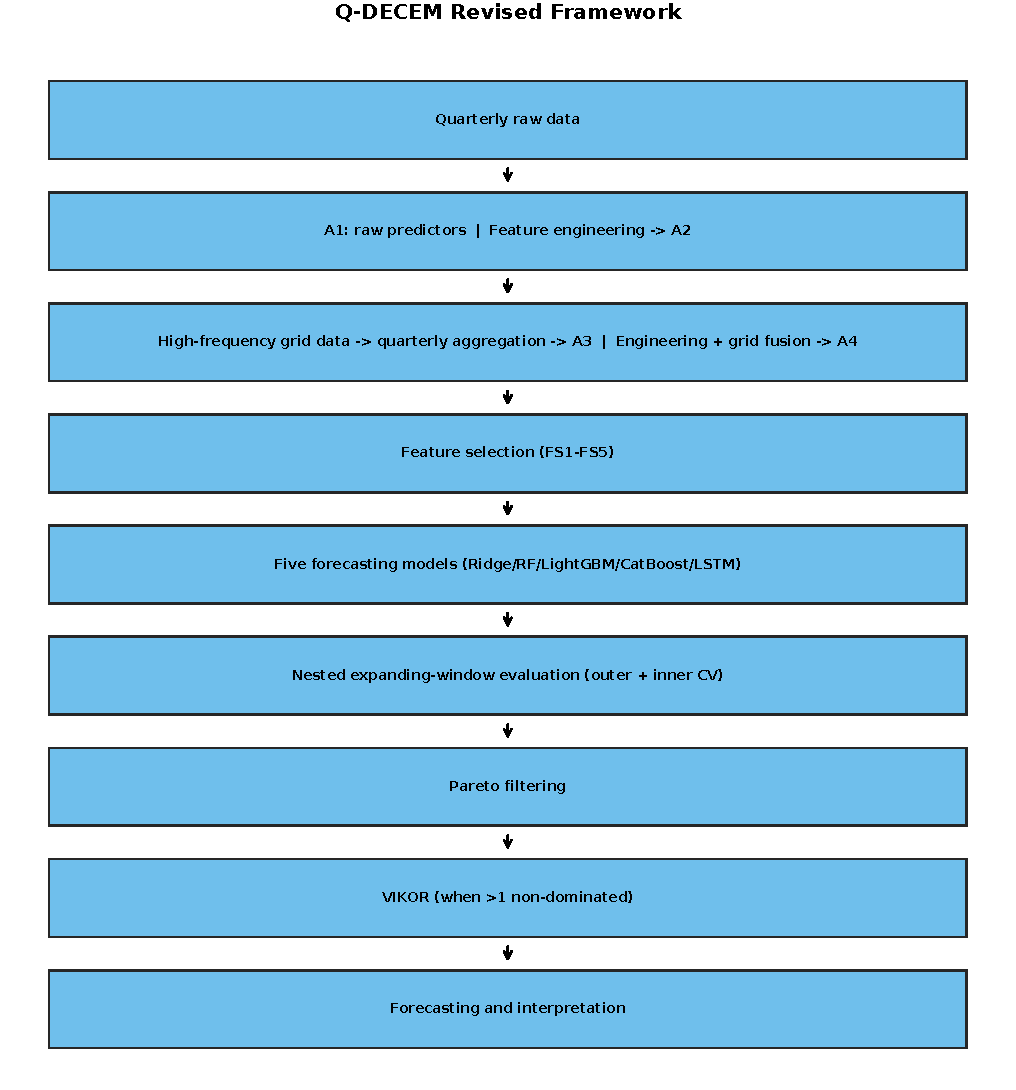
\includegraphics[width=0.95\linewidth,height=0.82\textheight,keepaspectratio]{figures/pdf/main/fig01_revised_qdecem_framework.pdf}
\caption{ \qdecem{} framework. The two streams share data governance, models, nested temporal validation, PSO optimisation, and decision criteria; they differ only in whether automated feature selection is applied.}
\label{fig:framework}
\end{figure}

\subsection{Study design and data chronology}

The target series contains quarterly UK \coo{} observations from 1999Q1 to 2025Q1 \citep{onsquarterlyghg2026}. Five macro-weather variables---GDP, population, mean air temperature, rainfall, and COVID-19 deaths---are joined to six quarterly mobility-shock variables. The mobility variables are quarterly means of the six Google categories as retail and recreation, grocery and pharmacy, parks, transit stations, workplaces, and residential locations \citep{googlemobility2022,googlemobilitydocumentation2022}. The source archive contains 974 daily UK-national observations from 15 February 2020 to 15 October 2022. Outside that interval, the mobility variables are assigned a neutral zero by design. This indicates that no Google-reported pandemic deviation is represented; it is not an observed statement that mobility exactly equalled its baseline.

Electricity information comes from the GB Carbon Intensity API and associated historical generation-mix data \citep{neso2026}. The retrieved grid record contains 34 complete quarters beginning in 2018Q1; two incomplete quarters are excluded by a 0.95 completeness threshold. Renewable and low-carbon electricity shares from Our World in Data (OWID) are annual and are lagged by one calendar year before entering any quarterly model \citep{owidrenewables2026,owidlowcarbon2026}. The observed target ends in 2025Q1, so later grid observations are retained for source validation but do not enter model evaluation. Section~\ref{sec:nowcast} uses this retained margin directly: real grid data already exist five quarters beyond the current target origin.

The primary comparison uses the common grid-covered panel. This keeps all A and B configurations on identical forecast dates. Under the common-period nested evaluation, 11 out-of-sample forecasts are available at the one-quarter horizon (H1), while eight are available at the two- and four-quarter horizons (H2 and H4), reflecting the shorter set of forecast origins for the longer horizons. A longer 1999--2025 panel remains informative for descriptive context, but it is not mixed with the common-period decision ranking because a longer training history would confound data-source effects with sample-length effects. Table~\ref{tab:data_blocks} summarises the information blocks used by the executable feature registry.

\begin{table}[H]
\centering
\caption{Predictor blocks, timing rules, and roles in the experiment.}
\label{tab:data_blocks}
\scriptsize
\begin{threeparttable}
\begin{tabularx}{\textwidth}{@{}p{1.7cm}p{4.4cm}p{0.8cm}p{3.0cm}Y@{}}
\toprule
Block & Variables & Count & Timing rule & Role \\
\midrule
Macro-weather & GDP, population, air temperature, rainfall, COVID-19 deaths & 5 & GDP delayed one quarter; other completed-quarter values & Baseline economic, demographic, climatic, and disruption context \\
Mobility shock & Retail/recreation, grocery/pharmacy, parks, transit, workplaces, residential & 6 & Quarterly mean; zero outside 2020-02-15--2022-10-15 archive & Represents pandemic-era behavioural disruption \\
Engineered & Four \coo{} lags, \coo{} log growth, GDP growth, lagged \coo{}/population, HDD, CDD, Q2--Q4, COVID and energy-crisis indicators & 14 & Target-derived terms lagged by at least one quarter & Adds persistence, seasonality, weather-demand proxies, and known regimes \\
Grid & Mean, p90 and SD of carbon intensity; high/low-intensity shares; renewable, low-carbon, fossil, gas and wind shares & 10 & Quarter retained only if completeness $\geq0.95$ & Represents within-quarter electricity-system conditions \\
Annual transition & Lagged OWID renewable and low-carbon electricity shares & 2 & Previous calendar year applied to current-year quarters & Adds conservative long-run transition context \\
\bottomrule
\end{tabularx}
\begin{tablenotes}[flushleft]\footnotesize
\item The 11-variable baseline combines the macro-weather and mobility blocks. Renewable and low-carbon shares are not synonymous: the latter includes nuclear generation.
\end{tablenotes}
\end{threeparttable}
\end{table}

\subsection{Leakage-controlled feature engineering}

The engineered block contains 14 variables. Four lags preserve the previous one to four quarters of \coo{}, with the fourth lag representing the same season one year earlier. Historical emissions growth is defined as
\begin{equation}
 \Delta\log y_{t-1}=\log(y_{t-1})-\log(y_{t-2}),
\end{equation}
so the current target $y_t$ never appears in the predictor. The population-scaled emissions indicator is also historical:
\begin{equation}
 I^{\mathrm{pop}}_t=\frac{y_{t-1}}{\mathrm{Population}_{t-1}}.
 \label{eq:intensity}
\end{equation}
GDP growth is calculated from release-available values. Heating- and cooling-degree proxies use an $18\,^{\circ}\mathrm{C}$ reference:
\begin{align}
 \mathrm{HDD}_t&=\max(0,18-\mathrm{AirTemp}_t),\\
 \mathrm{CDD}_t&=\max(0,\mathrm{AirTemp}_t-18).
\end{align}
Quarter indicators Q2--Q4 use Q1 as the reference. The COVID indicator covers 2020Q1--2021Q4 and the energy-crisis indicator 2022Q1--2023Q4.

Six engineered variables are target-derived as the four lags, historical log growth, and lagged \coo{} per population. They appear only in A2/A4 and their B-stream counterparts. The remaining configurations contain no target-derived predictors. This separation is important because the final winner can then be assessed without relying on transformed versions of the target.

Every variable is defined in a machine-readable registry recording its formula, source, release delay, minimum lag, target dependence, missing-value rule, and membership in A1--A4. The design matrix is built from this registry rather than from all merged columns. Figure~\ref{fig:governance} provides the visual audit trail, and the full 37-row registry is reproduced in Supplementary Table~S1.

\begin{figure}
\centering
\begin{adjustbox}{max width=\linewidth,max totalheight=0.88\textheight,center}
\begin{minipage}{18cm}
\centering
\figpanel{\linewidth}{a}{figures/pdf/main/fig02_predictor_governance_map.pdf}
\par\vspace{0.35cm}
\figpanel{\linewidth}{b}{figures/pdf/main/fig03_grid_aggregation_quality.pdf}
\end{minipage}
\end{adjustbox}
\caption{Predictor governance and external-data quality. Panel (a) maps target dependence, horizon safety, audit status, and configuration membership for all 37 candidates. Panel (b) reports quarterly completeness of the half-hourly grid record and the 0.95 inclusion threshold.}
\label{fig:governance}
\end{figure}

\subsection{Two streams and four information configurations}

The experiment is deliberately split before feature selection. Stream A asks what happens when each audited information set is retained in full. Stream B asks whether one of five selection strategies can improve the same four pools. Table~\ref{tab:configurations} gives the resulting eight families.

\begin{table}[H]
\centering
\caption{Two-stream configuration design.}
\label{tab:configurations}
\begin{tabularx}{\textwidth}{@{}p{0.8cm}p{1.2cm}p{4.2cm}p{1.7cm}Y@{}}
\toprule
Code & Stream & Candidate information & Audited count & Question answered \\
\midrule
A1 & No FS & Macro-weather + mobility & 11 & How far can the baseline information set forecast? \\
A2 & No FS & A1 + engineered variables & 25 & Does feature engineering add useful signal? \\
A3 & No FS & A1 + grid and lagged annual transition variables & 23 & Does electricity-system fusion add useful signal? \\
A4 & No FS & A1 + engineered + grid/transition variables & 37 & Does complete fusion outperform simpler pools? \\
B1 & With FS & A1 candidate pool + FS1--FS5 & 11 candidates & Does selection help a compact baseline pool? \\
B2 & With FS & A2 candidate pool + FS1--FS5 & 25 candidates & Can selection recover value from the engineered pool? \\
B3 & With FS & A3 candidate pool + FS1--FS5 & 23 candidates & Can selection preserve grid-fusion value with fewer variables? \\
B4 & With FS & A4 candidate pool + FS1--FS5 & 37 candidates & Can selection control the full-fusion dimensionality? \\
\bottomrule
\end{tabularx}
\end{table}

Every Stream A family is fitted with five models, producing 20 candidates. Every Stream B family is crossed with five selectors and five models, producing 100 candidates. The 20 Stream A candidates are ranked together; the 100 Stream B candidates are ranked together. Family-level best-accuracy models are reported for diagnosis, but they do not replace the global stream decision.

\subsection{Five feature-selection strategies}

Stream B uses five strategies that embody different definitions of relevance. FS1 is linear stability selection. A regularised linear estimator is fitted across inner expanding folds, and variables are evaluated through coefficient magnitude, sign consistency, and selection frequency. FS2 is wrapper selection. Recursive elimination, sequential forward selection, and sequential backward selection score subsets through inner-fold forecasting performance \citep{kohavi1997,guyon2003}. FS3 fits XGBoost inside each inner training fold and evaluates validation SHAP magnitude and rank stability. FS4 permutes each feature in the inner validation period and measures the resulting increase in error. FS5 is a vote-based consensus:
\begin{equation}
 V_j=\sum_{s=1}^{4}\mathbb{I}(j\in\mathcal{S}_s),
\end{equation}
with the primary rule retaining $V_j\geq3$. Alternative thresholds are examined as sensitivity settings.

Selection is repeated inside each outer training window. Outer test observations do not influence coefficients, wrapper subsets, SHAP values, permutation scores, vote thresholds, or subset rankings. Table~\ref{tab:experimental_setup} summarises the modelling and decision stages.

\begin{table}[H]
\centering
\caption{Forecasting, optimisation, validation, and decision settings.}
\label{tab:experimental_setup}
\begin{tabularx}{\textwidth}{@{}p{2.4cm}p{4.0cm}Y@{}}
\toprule
Stage & Primary implementation & Purpose \\
\midrule
Models & Ridge, random forest, LightGBM, CatBoost, LSTM & Compare regularised linear, bagged, boosted, and recurrent architectures \\
Optimisation & PSO; 20 particles, 30 iterations; model-specific parameter bounds & Tune every model within the inner temporal loop \\
Forecasting & Direct H1, H2, and H4 models & Avoid dependence on unknown future covariates and separate horizon behaviour \\
Validation & Nested expanding windows; common outer dates across all primary candidates & Prevent leakage in preprocessing, FS, and optimisation \\
Baselines & Previous-quarter and seasonal-naive forecasts & Establish whether MASE falls below a meaningful benchmark \\
Primary metric & MASE; horizon aggregate $0.50H1+0.30H2+0.20H4$ & Give greater weight to near-term accuracy without hiding longer horizons \\
Decision criteria & WMASE, worst-horizon MASE, fold-error dispersion, feature count, runtime & Balance accuracy, robustness, parsimony, and computational practicality \\
Decision method & Pareto filtering, then VIKOR; TOPSIS and weighted-sum sensitivity & Select a transparent compromise rather than a single-metric winner \\
Statistical confirmation & Wilcoxon signed-rank and Diebold--Mariano tests on paired forecast errors, Holm--Bonferroni corrected & Confirm pooled significance holds at the individual-horizon level, accounting for serial correlation in multi-step errors \\
Interpretation & Model-appropriate SHAP/importance; pre-, during-, and post-COVID regimes; within-family statistic decomposition & Examine what information drives the selected forecasts, and whether a leading statistic's attribution share reflects joint or standalone value \\
\bottomrule
\end{tabularx}
\end{table}

\subsection{Models and PSO optimisation}

Ridge regression provides a regularised linear benchmark \citep{hoerl1970}. Random forest represents bagged nonlinear trees \citep{breiman2001}. LightGBM and CatBoost represent two different gradient-boosting designs: leaf-wise histogram boosting and ordered symmetric-tree boosting, respectively \citep{ke2017,prokhorenkova2018}. LSTM represents a recurrent sequence architecture that can learn temporal dependence but requires substantially more data to estimate reliably \citep{hochreiter1997}.

PSO tunes every model within the inner expanding windows. A particle encodes a candidate hyperparameter vector and is evaluated by mean inner-fold MASE. Search spaces cover the Ridge penalty; tree count and depth for random forest; learning rate, depth or leaves, and boosting iterations for LightGBM and CatBoost; and units, dropout, learning rate, and lookback for LSTM. The LSTM prediction routine carries the final lookback observations from the training history into the forecast window and raises an error when prediction length or dates do not match the targets, preventing silent broadcasting or truncation.

\subsection{Nested evaluation and metrics}

In outer fold $k$, observations available at origin $t_k$ form the training set and $y_{t_k+h}$ remains untouched until the final prediction. Inside the training set, expanding folds are used for feature selection and PSO. Scaling and any training-relative threshold are recomputed from scratch. The sequence is therefore
\begin{equation*}
\text{outer training}\rightarrow\text{inner preprocessing/FS/PSO}\rightarrow
\text{refit}\rightarrow\text{outer forecast}.
\end{equation*}

The primary measure is mean absolute scaled error \citep{hyndmankoehler2006}:
\begin{equation}
 \mathrm{MASE}_h=
 \frac{n_h^{-1}\sum_{i=1}^{n_h}|y_i-\widehat{y}_i|}
 {(T-4)^{-1}\sum_{t=5}^{T}|y_t-y_{t-4}|}.
 \label{eq:mase}
\end{equation}
A value below one indicates lower error than the seasonal-naive scale. The three horizons are combined as
\begin{equation}
 \mathrm{WMASE}=0.50\,\mathrm{MASE}_{H1}+0.30\,\mathrm{MASE}_{H2}+0.20\,\mathrm{MASE}_{H4}.
 \label{eq:wmase}
\end{equation}
MAE, RMSE, sMAPE, and $R^2$ remain complementary outputs. The worst-horizon MASE is retained separately, and temporal dispersion is measured from fold-level errors.

Paired configuration comparisons use common outer folds. Two tests are reported side by side, each suited to a different assumption. The Wilcoxon signed-rank test treats paired absolute-error differences as exchangeable and is appropriate for the short, non-normal samples available here. The Diebold--Mariano test \citep{dieboldmariano1995} instead models the paired loss differential directly, with an autocovariance-based long-run variance estimate truncated at lag $h-1$ and the Harvey--Leybourne--Newbold small-sample correction -- appropriate because an $h$-step-ahead forecast error can carry up to $(h-1)$-order serial correlation that a simple rank test does not accommodate. Both are Holm--Bonferroni corrected within their own family of tests. The Diebold--Mariano estimator is reported only at $H1$ and $H2$: at $H4$, with eight paired origins and a lag truncation of three, the long-run variance estimate is not reliably positive, and the test is reported as undefined rather than forced to a number that the sample cannot support.

\subsection{Pareto--VIKOR selection and interpretation}

A candidate is Pareto dominated when another is no worse on every decision criterion and better on at least one. Only non-dominated candidates enter VIKOR. For alternative $i$, the weighted aggregate gap $S_i$, maximum regret $R_i$, and compromise score $Q_i$ follow \citet{opricovic2004,opricovic2007}. Equal weights are the primary specification, with accuracy, horizon robustness, stability, parsimony, and runtime emphasis used for sensitivity analysis. Lower $Q_i$ is preferred. Exact ties are resolved through deterministic secondary sorting rather than integer truncation.

The procedure is applied separately to Stream A and Stream B, then once more to the two finalists. Interpretability focuses on the selected unrestricted model, the selected feature-screened model, and the overall winner. Tree models use TreeSHAP \citep{lundberg2017}; cross-model rank profiles supplement model-specific explanations. Regimes are defined as pre-COVID (before 2020Q1), COVID (2020Q1--2021Q4), and post-COVID (from 2022Q1). A regime result is reported only when the saved attribution output is non-degenerate.

For tree-based finalists, predictive attribution is computed from the actual PSO-tuned refits rather than library-default estimators, since a refit that does not match the tuned model used for forecasting can materially misrepresent which features the champion actually uses. TreeSHAP outputs are subjected to automated integrity checks for all-zero attributions, duplicated regime profiles, feature-order mismatches, missing or infinite values, observation-count mismatches, and SHAP additivity. All reported finalist-regime combinations pass these checks, with prediction reconstruction error at machine precision. Regime comparisons therefore use validated mean absolute SHAP values for pre-COVID, COVID and post-COVID observations; they are interpreted as predictive attribution rather than causal effects.

Beyond the champion's full 23-feature attribution, a within-family decomposition isolates each of the five carbon-intensity statistics (mean, 90th percentile, standard deviation, and the high- and low-intensity settlement-period shares) as the sole grid predictor added to the raw-plus-mobility baseline, alongside the already-reported carbon-intensity-family and generation-mix-family ablations. This separates a statistic's attribution share inside the joint model from its predictive value in isolation -- two quantities that a single SHAP summary cannot distinguish on its own. Section~\ref{sec:nowcast} extends the framework operationally: the champion's tuned direct-horizon models are re-fit on all available history and applied to the true current forecast origin, and empirical leave-one-out prediction intervals are constructed from the champion's own historical residuals at each horizon.

\section{Results}\label{sec:results}

\subsection{The audit changed the question before the models were compared}

The first result is methodological. The registry contains 37 candidate predictors and identifies exactly six as target-derived: four \coo{} lags, historical \coo{} growth, and lagged \coo{} per population. All six have a minimum lag of at least one quarter and appear only in A2/A4. The winning A3 configuration therefore contains no transformed historical target variable. This matters because a contemporaneous intensity ratio could otherwise produce artificially strong forecasts. The design makes the final comparison about external information rather than disguised target recovery.

The external feeds also pass a transparent quality threshold. The mobility archive contains 974 daily observations but ends in October 2022. The grid feed contributes 34 complete quarters, with two incomplete quarters excluded. The annual OWID series are lagged by one year. Table~\ref{tab:source_quality} records these limitations rather than hiding them inside preprocessing.

\begin{table}[!htbp]
\centering
\scriptsize
\setlength{\tabcolsep}{3.5pt}
\renewcommand{\arraystretch}{0.92}
\caption{External-source coverage and data-quality controls.}
\label{tab:source_quality}
\begin{tabularx}{\textwidth}{@{}p{3.1cm}p{2.0cm}p{2.0cm}p{1.4cm}Y@{}}
\toprule
Source & First observation & Last observation & Records & Coverage and governance note \\
\midrule
Google COVID-19 mobility & 2020-02-15 & 2022-10-15 & 974 daily & UK national series; quarterly means; neutral-zero convention outside archive \\
NESO GB Carbon Intensity API & 2018Q1 & 2026Q2 retrieved & 34 quarters & Two quarters excluded below 0.95 completeness; modelling target ends 2025Q1; the 2025Q2--2026Q2 margin is used directly in Section~\ref{sec:nowcast} \\
OWID renewable share & Annual series & Retrieved 2026-08-01 & -- & One-year lag before quarterly use \\
OWID low-carbon share & Annual series & Retrieved 2026-08-01 & -- & One-year lag before quarterly use \\
\bottomrule
\end{tabularx}
\end{table}

\subsection{Stream A: the grid-only extension leads the unrestricted comparison}

\begin{table}[H]
\centering
\caption{Stream A results for all 20 unrestricted candidates. Lower MASE and rank are better.}
\label{tab:streamA}
\scriptsize
\setlength{\tabcolsep}{4pt}
\renewcommand{\arraystretch}{0.85}
\begin{adjustbox}{max width=\textwidth}
\begin{tabular}{@{}llrrrrrl@{}}
\toprule
Config. & Model & WMASE & H1 & H2 & H4 & Rank & Pareto status \\
\midrule
A3 & LightGBM & \textbf{0.454} & \textbf{0.376} & 0.575 & 0.467 & 1 & Non-dominated \\
A3 & CatBoost & 0.623 & 0.667 & 0.587 & 0.566 & 2 & Non-dominated \\
A3 & Random forest & 0.683 & 0.694 & 0.717 & 0.606 & 3 & Non-dominated \\
A2 & Random forest & 0.720 & 0.717 & 0.748 & 0.688 & 4 & Non-dominated \\
A1 & Random forest & 0.747 & 0.851 & 0.772 & 0.450 & 5 & Non-dominated \\
A2 & Ridge & 0.734 & 0.812 & 0.567 & 0.788 & 6 & Non-dominated \\
A1 & Ridge & 0.905 & 0.985 & 0.739 & 0.954 & 7 & Non-dominated \\
A1 & CatBoost & 0.629 & 0.677 & 0.556 & 0.621 & 8 & Non-dominated \\
A4 & CatBoost & 0.615 & 0.719 & \textbf{0.515} & 0.503 & 9 & Non-dominated \\
A3 & Ridge & 0.839 & 0.995 & 0.574 & 0.849 & 10 & Non-dominated \\
A4 & Random forest & 0.699 & 0.665 & 0.726 & 0.746 & 11 & Non-dominated \\
A1 & LSTM & 1.020 & 1.020 & 0.990 & 1.065 & 12 & Non-dominated \\
A4 & Ridge & 0.706 & 0.792 & 0.538 & 0.744 & 13 & Non-dominated \\
A1 & LightGBM & 0.761 & 0.854 & 0.751 & 0.544 & 14 & Non-dominated \\
A3 & LSTM & 1.018 & 1.022 & 0.973 & 1.077 & 15 & Non-dominated \\
A4 & LightGBM & 0.722 & 0.791 & 0.778 & \textbf{0.465} & 16 & Non-dominated \\
A2 & LSTM & 0.710 & 0.711 & 0.673 & 0.765 & -- & Dominated \\
A2 & CatBoost & 0.722 & 0.737 & 0.709 & 0.706 & -- & Dominated \\
A2 & LightGBM & 0.933 & 1.101 & 0.730 & 0.817 & -- & Dominated \\
A4 & LSTM & 0.949 & 0.885 & 0.944 & 1.118 & -- & Dominated \\
\bottomrule
\end{tabular}
\end{adjustbox}
\end{table}

The unrestricted comparison contains 20 model--configuration candidates. Sixteen are non-dominated and four are removed: A2/LightGBM, A2/CatBoost, A2/LSTM, and A4/LSTM. The ranking is not driven by model class alone. The first three positions all come from A3, the core-plus-grid pool: LightGBM, CatBoost, and random forest. A3/LightGBM is the clear winner with WMASE 0.454 and horizon-specific MASE of 0.376, 0.575, and 0.467 (Table~\ref{tab:streamA}). Its one-quarter forecast reduces scaled error by about 62\% relative to the MASE=1 seasonal-naive benchmark.

The pattern is easier to see in Figure~\ref{fig:global_comparison}. For every model except LSTM, A3 performs better than the engineered-only A2 pool. A4, despite containing all 37 predictors, does not improve on A3. Its strongest candidate, CatBoost, reaches WMASE 0.615 but remains behind A3/LightGBM. The result is not that engineered variables are intrinsically uninformative. Rather, on this short common panel, their added dimensionality does not complement the grid signal enough to compensate for the extra estimation burden.

LSTM provides a useful counterexample to the assumption that temporal complexity must help a time series. Its WMASE is approximately one or worse in A1, A3, and A4, and the A4 version is dominated. The series provides too few common-period observations for a recurrent architecture to learn a stable multivariate sequence, even after PSO tuning. Tree boosting is better matched to the tabular, mixed-source structure.

\clearpage
\pagestyle{empty}
\begin{landscape}
\AddToShipoutPictureFG{\landscapepagenumber}
\begin{figure}[p]
\centering
\begin{adjustbox}{max width=\linewidth,max totalheight=0.88\textheight,center}
\begin{minipage}{0.96\linewidth}
\centering
\figpanel{0.48\linewidth}{a}{figures/pdf/main/fig03a_stream_A_global_comparison.pdf}\hfill
\figpanel{0.48\linewidth}{b}{figures/pdf/main/fig03b_stream_B_global_overview.pdf}
\par\vspace{0.35cm}
\figpanel{0.48\linewidth}{c}{figures/pdf/main/fig03c_stream_B_shortlist_magnified.pdf}\hfill
\figpanel{0.48\linewidth}{d}{figures/pdf/main/fig03d_best_A_vs_best_B.pdf}
\end{minipage}
\end{adjustbox}
\caption{Global comparison across the two streams. Panel (a) reports all 20 unrestricted candidates. Panel (b) reports all 100 feature-selected candidates. Panel (c) magnifies the Stream B Pareto shortlist. Panel (d) compares the two stream finalists after criterion normalisation.}
\label{fig:global_comparison}
\end{figure}
\end{landscape}
\ClearShipoutPictureFG
\pagestyle{plain}

\subsection{Stream B: selection creates a compact winner, but the most accurate subsets still contain grid information}

Stream B expands the search to 100 candidates. Forty-eight are non-dominated and 52 are removed. Equal-weight VIKOR selects B1/FS1/CatBoost: six variables---GDP, population, air temperature, rainfall, COVID-19 deaths, and parks mobility---with WMASE 0.655. The choice is not the most accurate feature-selected model. B3/FS2/LightGBM reaches WMASE 0.506 with 15 variables, and B3/FS1/LightGBM reaches 0.518 with 11. The six-variable CatBoost wins because it combines lower feature count and lower fold-error dispersion with acceptable accuracy.

Table~\ref{tab:streamB} shows the leading non-dominated alternatives. The contrast between ranks 1, 2, and 10 is central to the paper. The first-ranked model is the best compromise under equal weights; the tenth-ranked B3 wrapper model is the best accuracy-only family winner in Stream B. A decision maker focused almost entirely on accuracy would choose the latter. A decision maker valuing compactness and stability more evenly would choose the former.

\begin{table}[!htbp]
\centering
\caption{Leading Stream B candidates in equal-weight VIKOR order. The complete 100-candidate table is Supplementary Table S3.}
\label{tab:streamB}
\footnotesize
\begin{adjustbox}{max width=\textwidth}
\begin{tabular}{@{}rlllrrrrr@{}}
\toprule
Rank & Pool & FS & Model & Features & WMASE & H1 & H2 & H4 \\
\midrule
1 & B1 & Linear stability & CatBoost & 6 & 0.655 & 0.697 & 0.597 & 0.637 \\
2 & B3 & Linear stability & LightGBM & 11 & 0.518 & 0.579 & 0.532 & 0.346 \\
3 & B2 & XGBoost--SHAP & CatBoost & 5 & 0.689 & 0.633 & 0.800 & 0.661 \\
4 & B3 & XGBoost--SHAP & Random forest & 6 & 0.692 & 0.760 & 0.616 & 0.637 \\
5 & B1 & Wrapper & CatBoost & 11 & 0.629 & 0.677 & 0.556 & 0.621 \\
6 & B2 & XGBoost--SHAP & Random forest & 5 & 0.729 & 0.694 & 0.821 & 0.675 \\
7 & B3 & Linear stability & Random forest & 11 & 0.703 & 0.764 & 0.621 & 0.674 \\
8 & B3 & Linear stability & CatBoost & 11 & 0.650 & 0.727 & 0.510 & 0.670 \\
9 & B2 & XGBoost--SHAP & Ridge & 5 & 0.863 & 0.930 & 0.712 & 0.923 \\
10 & B3 & Wrapper & LightGBM & 15 & \textbf{0.506} & \textbf{0.486} & 0.640 & \textbf{0.356} \\
11 & B1 & XGBoost--SHAP & Ridge & 5 & 0.880 & 0.950 & 0.715 & 0.954 \\
12 & B1 & Linear stability & Ridge & 6 & 0.880 & 0.949 & 0.716 & 0.951 \\
13 & B3 & XGBoost--SHAP & Ridge & 6 & 0.855 & 0.939 & 0.666 & 0.930 \\
14 & B3 & Wrapper & Random forest & 15 & 0.719 & 0.747 & 0.730 & 0.634 \\
15 & B3 & Wrapper & CatBoost & 15 & 0.646 & 0.735 & 0.489 & 0.657 \\
\bottomrule
\end{tabular}
\end{adjustbox}
\end{table}

The selectors also behave differently at the factor level. Wrapper selection has the best mean WMASE, 0.790, but the widest rank dispersion. Permutation stability is consistently weakest, with mean WMASE 1.060 and a median above the naive threshold. It repeatedly chooses a narrow, mobility-heavy subset that does not transfer well across models or configurations. CatBoost has the best mean and median performance across model occurrences, while LSTM is weakest. Table~\ref{tab:factor_summary} places these averages in context; they describe tendencies, not the final decision.

\begin{table}[!htbp]
\centering
\caption{Global factor-level summary across all candidates carrying each factor.}
\label{tab:factor_summary}
\footnotesize
\begin{adjustbox}{max width=\textwidth}
\begin{tabular}{@{}llrrrr@{}}
\toprule
Factor type & Level & Candidates & Mean WMASE & Median WMASE & Median rank \\
\midrule
Configuration & A1 & 30 & 0.864 & 0.880 & 19.0 \\
 & A2 & 30 & 0.893 & 0.870 & 21.0 \\
 & A3 & 30 & \textbf{0.806} & \textbf{0.793} & \textbf{14.0} \\
 & A4 & 30 & 0.858 & 0.883 & 22.0 \\
B family & B1 & 25 & 0.874 & 0.880 & 29.5 \\
 & B2 & 25 & 0.918 & 0.907 & 25.5 \\
 & B3 & 25 & \textbf{0.823} & \textbf{0.811} & \textbf{15.5} \\
 & B4 & 25 & 0.882 & 0.886 & 34.5 \\
FS strategy & Linear stability & 20 & 0.840 & 0.852 & 14.5 \\
 & Wrapper & 20 & \textbf{0.790} & \textbf{0.754} & 33.0 \\
 & XGBoost--SHAP & 20 & 0.834 & 0.836 & 16.0 \\
 & Permutation stability & 20 & 1.060 & 1.041 & 30.0 \\
 & Consensus & 20 & 0.848 & 0.815 & 31.0 \\
Model & Ridge & 24 & 0.870 & 0.871 & 18.5 \\
 & Random forest & 24 & 0.806 & 0.745 & 7.0 \\
 & LightGBM & 24 & 0.845 & 0.819 & 16.0 \\
 & CatBoost & 24 & \textbf{0.767} & \textbf{0.688} & 8.5 \\
 & LSTM & 24 & 0.988 & 1.021 & 33.5 \\
\bottomrule
\end{tabular}
\end{adjustbox}
\end{table}

Feature membership explains why B3 remains competitive. GDP, population, air temperature, rainfall, and parks mobility form a recurring core across the four candidate pools. In B3, Grid-CI-std, Grid-CI-high-share, and Grid-gas-share receive three of four primary-method votes. By contrast, several average mix variables receive little support. The selection evidence therefore points to the distribution and extremes of grid carbon intensity, rather than the quarterly mean fuel mix alone, as the most robust addition.

The engineered pool produces a different picture. CO$_2$ lag 2 and lag 4 receive support, but lag 1, lag 3, historical intensity, CDD, and the energy-crisis dummy are weak or unanimously rejected in some pools. When all 37 variables compete in B4, no feature receives more than two of four votes. The signal becomes fragmented rather than strengthened. Figure~\ref{fig:membership} collects the four membership matrices, and Supplementary Table~S4 provides all 96 feature-level decisions.

\begin{figure}
\centering
\begin{adjustbox}{max width=\linewidth,max totalheight=0.88\textheight,center}
\begin{minipage}{18cm}
\centering
\figpanel{8.8cm}{a}{figures/pdf/main/fig08_b1_feature_selection_membership.pdf}\hfill
\figpanel{8.8cm}{b}{figures/pdf/main/fig08_b2_feature_selection_membership.pdf}
\par\vspace{0.35cm}
\figpanel{8.8cm}{c}{figures/pdf/main/fig08_b3_feature_selection_membership.pdf}\hfill
\figpanel{8.8cm}{d}{figures/pdf/main/fig08_b4_feature_selection_membership.pdf}
\end{minipage}
\end{adjustbox}
\caption{Feature-selection membership in B1--B4. Dark cells indicate retention by the named strategy. The final column is the vote-based consensus.}
\label{fig:membership}
\end{figure}

\begin{table}[H]
\centering
\caption{Feature-selection agreement: recurring core signals and notable rejections.}
\label{tab:fs_summary}
\begin{tabularx}{\textwidth}{@{}p{1.0cm}p{6.5cm}Y@{}}
\toprule
Pool & Highest cross-method support & Notable weak or unanimous rejections \\
\midrule
B1 & GDP, population, air temperature, rainfall, parks mobility, transit mobility & Retail/recreation receives only one vote \\
B2 & Parks mobility, \coo{} lag 2, \coo{} lag 4; broader two-vote band for macro, GDP growth, HDD, Q2/Q4 & \coo{} lag 3, \coo{}/population, CDD, energy-crisis indicator receive zero votes \\
B3 & GDP, population, air temperature, rainfall, Grid-CI-std, Grid-CI-high-share, Grid-gas-share & Several mobility series and Grid-CI-low-share receive zero votes \\
B4 & Mixed two-vote group spanning GDP, selected lags, GDP growth, seasonal and grid-intensity features & No variable reaches three votes; six variables receive zero votes, indicating fragmented agreement \\
\bottomrule
\end{tabularx}
\end{table}

\subsection{The final decision favours accuracy, but the compact alternative remains informative}

The final comparison is direct. Best-A is A3/LightGBM with all 23 core-plus-grid variables. Best-B is B1/linear-stability/CatBoost with six variables. Best-A has lower MASE at every horizon and also lower runtime in the saved run. Best-B uses approximately one quarter of the variables and has lower fold-error dispersion. Equal-weight VIKOR gives Best-A $Q=0$ and Best-B $Q=0.5$, selecting Best-A overall (Table~\ref{tab:finalists}).

\begin{table}[!htbp]
\centering
\caption{Stream winners and final cross-stream decision.}
\label{tab:finalists}
\begin{adjustbox}{max width=\textwidth}
\begin{tabular}{@{}llllrrrrrrr@{}}
\toprule
Winner & Pool & FS & Model & Features & H1 & H2 & H4 & WMASE & Error SD & Runtime (s) \\
\midrule
Best-A / Overall & A3 & None & LightGBM & 23 & \textbf{0.376} & \textbf{0.575} & \textbf{0.467} & \textbf{0.454} & 1610.9 & \textbf{0.264} \\
Best-B & B1 & Linear & CatBoost & 6 & 0.697 & 0.597 & 0.637 & 0.655 & \textbf{982.5} & 12.461 \\
\bottomrule
\end{tabular}
\end{adjustbox}
\end{table}

The difference is largest at H1, where Best-A's MASE is 0.376 against 0.697. At H2 the finalists nearly converge, 0.575 against 0.597. At H4 the grid model regains a clear advantage, 0.467 against 0.637. The out-of-sample trajectories in Figure~\ref{fig:forecasts} show why one aggregate number is insufficient: the models face different residual patterns across the limited evaluation dates, and H2 is specifically the champion's weakest horizon.

\begin{figure}
\centering
\begin{adjustbox}{max width=\linewidth,max totalheight=0.88\textheight,center}
\begin{minipage}{18cm}
\centering
\figpanel{8.8cm}{a}{figures/pdf/forecasting/fig_best_overall_forecast_H1.pdf}\hfill
\figpanel{8.8cm}{b}{figures/pdf/forecasting/fig_best_A_vs_B_forecast_H1.pdf}
\par\vspace{0.25cm}
\figpanel{8.8cm}{c}{figures/pdf/forecasting/fig_best_overall_forecast_H2.pdf}\hfill
\figpanel{8.8cm}{d}{figures/pdf/forecasting/fig_best_A_vs_B_forecast_H2.pdf}
\par\vspace{0.25cm}
\figpanel{8.8cm}{e}{figures/pdf/forecasting/fig_best_overall_forecast_H4.pdf}\hfill
\figpanel{8.8cm}{f}{figures/pdf/forecasting/fig_best_A_vs_B_forecast_H4.pdf}
\end{minipage}
\end{adjustbox}
\caption{Out-of-sample forecasts of the overall winner and direct finalist comparisons. Each row reports one forecast horizon: H1 in panels (a)--(b), H2 in panels (c)--(d), and H4 in panels (e)--(f). The left column shows the selected A3/LightGBM model; the right column places Best-A and Best-B on common dates.}
\label{fig:forecasts}
\end{figure}

\clearpage
\pagestyle{empty}
\begin{landscape}
\AddToShipoutPictureFG{\landscapepagenumber}
\begin{figure}[p]
\centering
\begin{adjustbox}{max width=\linewidth,max totalheight=0.88\textheight,center}
\begin{minipage}{0.96\linewidth}
\centering
\figpanel{0.48\linewidth}{a}{figures/pdf/main/fig11a_stream_A_pareto_frontier.pdf}\hfill
\figpanel{0.48\linewidth}{b}{figures/pdf/main/fig11b_stream_B_pareto_frontier.pdf}
\par\vspace{0.35cm}
\figpanel{0.48\linewidth}{c}{figures/pdf/main/fig14a_mcda_rank_sensitivity_stream_A.pdf}\hfill
\figpanel{0.48\linewidth}{d}{figures/pdf/main/fig14b_mcda_rank_sensitivity_stream_B.pdf}
\end{minipage}
\end{adjustbox}
\caption{Pareto structure and MCDM sensitivity. Stream A has a visually distinct accuracy leader and comparatively stable ranking; Stream B contains a denser trade-off frontier and greater sensitivity to criterion weights.}
\label{fig:decision_sensitivity}
\end{figure}
\end{landscape}
\ClearShipoutPictureFG
\pagestyle{plain}

The decision is robust in Stream A. Five of seven alternative schemes retain A3/LightGBM as the leading model; only a strong parsimony emphasis changes the winner to A1/CatBoost. Stream B is less stable. Only stability- and parsimony-emphasis variants agree with equal-weight VIKOR's B1/CatBoost choice, while accuracy- and horizon-emphasis variants prefer B3/linear/LightGBM. The uncertainty is not a flaw in the decision analysis; it reveals that Stream B contains several genuinely different compromises. Figure~\ref{fig:decision_sensitivity} combines the Pareto and rank-sensitivity views.

\subsection{What the champion learned from electricity-grid dynamics}\label{sec:shap}

Reproducing the A3/LightGBM champion under its tuned hyperparameters yields WMASE 0.4541, with H1, H2 and H4 MASE of 0.3763, 0.5751 and 0.4672, respectively -- unchanged from Table~\ref{tab:finalists} to three decimal places, confirming that the champion's attribution is computed from the same model that produced its forecasts. The global profile is strongly grid-centred. \texttt{Grid\_CI\_std} is the leading predictor and accounts for 31.8\% of total mean absolute SHAP attribution, followed by \texttt{Grid\_CI\_mean} (10.8\%) and \texttt{Grid\_CI\_p90} (9.0\%). \texttt{COVID\_Deaths} (7.4\%) and population (7.2\%) complete the top five. Air temperature, which appeared prominent in the earlier cross-model summary, ranks below these variables in the champion-specific explanation. The main signal is therefore not simply the average carbon intensity of electricity generation, but the within-quarter distribution of carbon intensity, particularly its dispersion, level and upper tail -- a description of what the model attributes weight to, not yet an answer to whether that weight reflects a joint or a standalone property; Section~\ref{sec:decomposition} tests that distinction directly.

This ordering is temporally stable. \texttt{Grid\_CI\_std} ranks first in the pre-COVID ($n=7$), COVID ($n=8$) and post-COVID ($n=13$) regimes. Grid-family predictors account for 69.0\%, 61.1\% and 67.7\% of total attribution across the three periods, while pairwise Spearman correlations of feature ranks range from 0.915 to 0.965. The evidence therefore does not support a large pandemic-era reshuffling of the champion's predictive hierarchy. Instead, grid dynamics remain the dominant information family throughout the observed period.

Best-B remains useful as a contrasting compact model because it relies on six non-grid variables and sacrifices some accuracy for parsimony and lower fold-level variability. Its interpretation should be retained only as a secondary comparison; the primary interpretive claim comes from the validated A3/LightGBM champion. Table~\ref{tab:regimes} and Figure~\ref{fig:importance} summarise the champion results.

\begin{table}[!htbp]
\centering
\caption{A3/LightGBM champion interpretation across regimes.}
\label{tab:regimes}
\begin{tabularx}{\columnwidth}{@{}p{1.7cm}p{0.8cm}Yp{2.0cm}@{}}
\toprule
Regime & $n$ & Ranked top five predictors & Grid-family share \\
\midrule
Pre-COVID & 7 & \texttt{Grid\_CI\_std}, \texttt{Grid\_CI\_mean}, \texttt{Grid\_CI\_p90}, population, \texttt{COVID\_Deaths} & 69.0\% \\
COVID & 8 & \texttt{Grid\_CI\_std}, GDP, workplaces mobility, \texttt{Grid\_CI\_p90}, \texttt{COVID\_Deaths} & 61.1\% \\
Post-COVID & 13 & \texttt{Grid\_CI\_std}, \texttt{Grid\_CI\_mean}, \texttt{COVID\_Deaths}, \texttt{Grid\_CI\_p90}, population & 67.7\% \\
\bottomrule
\end{tabularx}
\begin{minipage}{\columnwidth}
\footnotesize\textit{Note:} Grid-family share combines grid carbon-intensity and generation-mix predictors. Pairwise Spearman correlations of all 23 feature ranks are 0.921 (pre-COVID/COVID), 0.965 (pre-COVID/post-COVID), and 0.915 (COVID/post-COVID).
\end{minipage}
\end{table}

\begin{figure}[p]
\centering
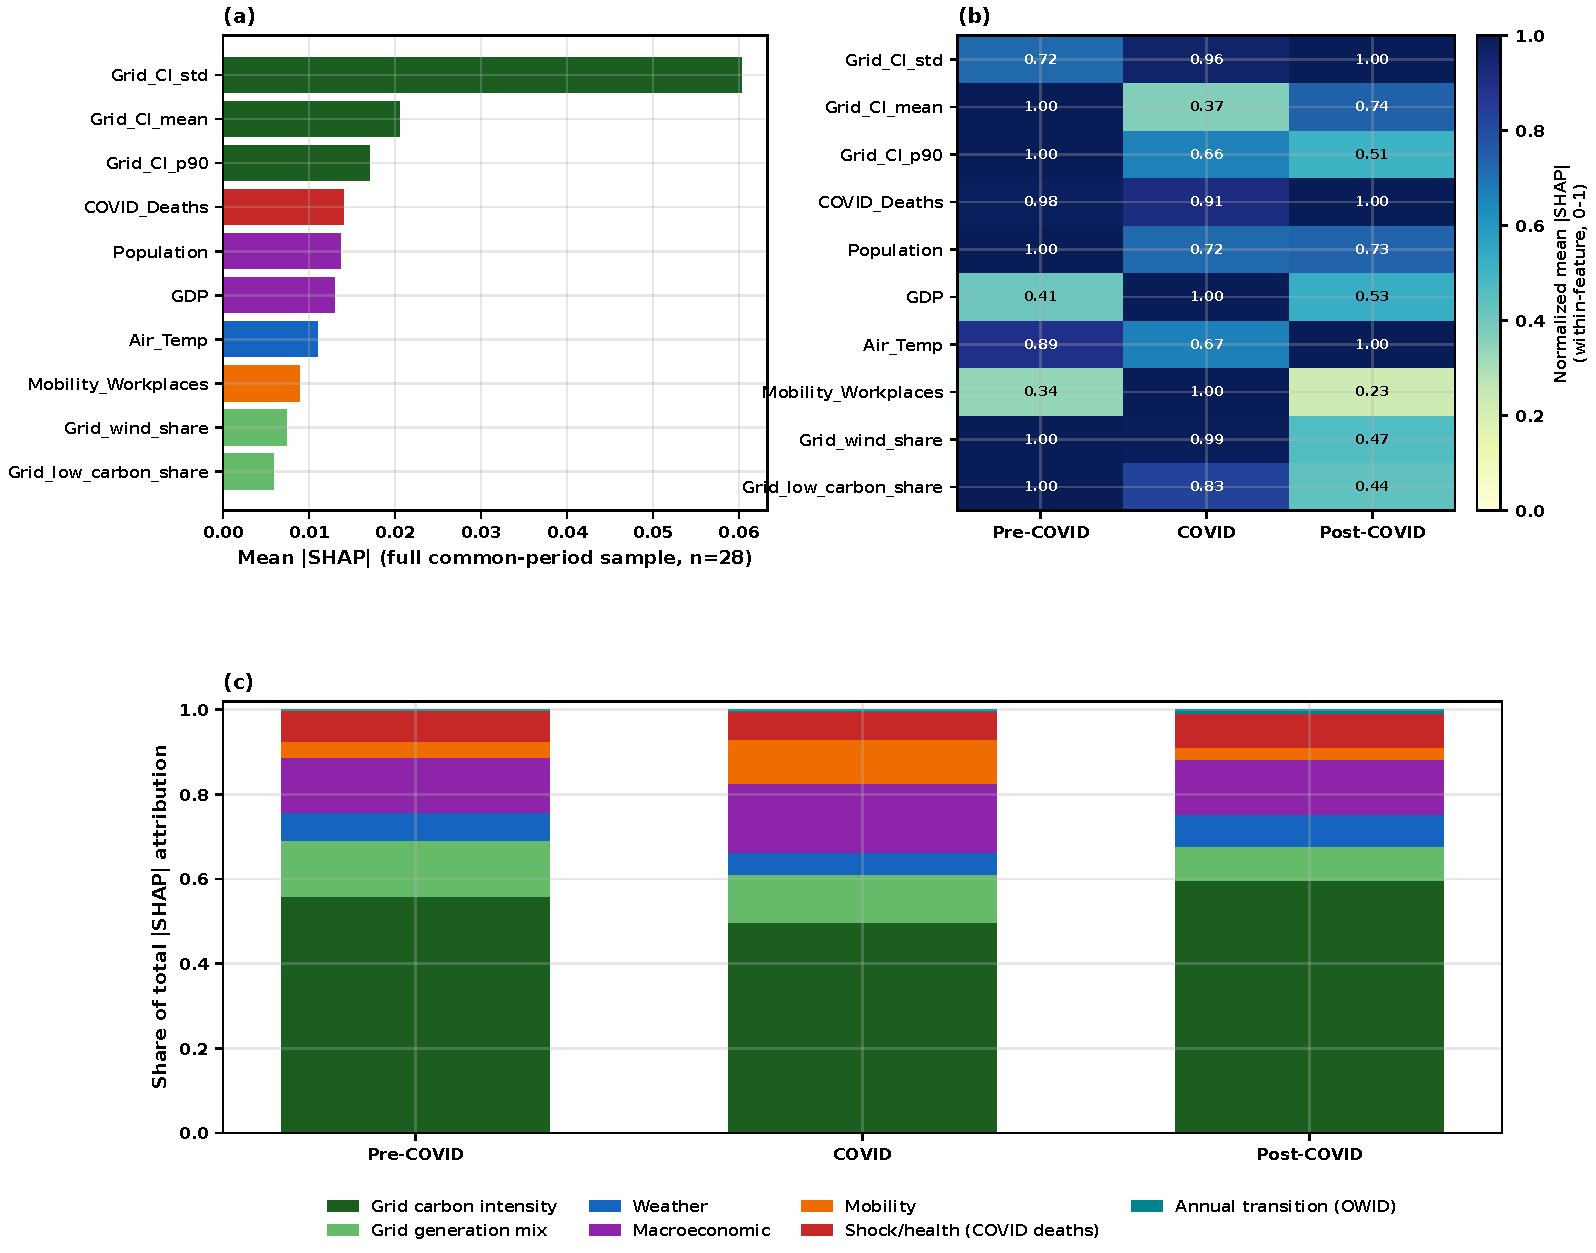
\includegraphics[width=0.98\textwidth,height=0.82\textheight,keepaspectratio]{figures/pdf/main/fig_champion_regime_importance.pdf}
\caption{Champion SHAP and regime interpretation. Panel (a) reports global mean absolute SHAP attribution for the tuned A3/LightGBM champion. Panel (b) compares normalized feature importance across pre-COVID, COVID, and post-COVID regimes. Panel (c) reports each predictor family's share of total absolute attribution within each regime.}
\label{fig:importance}
\end{figure}

\subsection{Decomposing the carbon-intensity family: attribution share is not standalone value}\label{sec:decomposition}

Section~\ref{sec:shap}'s attribution profile describes what the champion uses inside the full 23-feature model. It does not, on its own, establish whether \texttt{Grid\_CI\_std}'s leading share reflects genuine standalone predictive value or the marginal contribution it makes once the mean and upper tail are already present. To separate these, each of the five carbon-intensity statistics is added, alone, to the raw-plus-mobility baseline, alongside the combined five-statistic and no-grid reference points already reported in Table~\ref{tab:grid_robustness}.

Table~\ref{tab:decomposition} and Figure~\ref{fig:decomposition} give the answer directly. Tested alone, \texttt{Grid\_CI\_mean} (WMASE 0.598) is the strongest single carbon-intensity statistic, ahead of the low-intensity share (0.614) and the 90th percentile (0.621). \texttt{Grid\_CI\_std} alone reaches only 0.662 -- worse than every other individual statistic tested, and worse than the no-grid baseline itself (0.637). The high-intensity share performs worst alone (0.709). \textbf{Dispersion's 31.8\% attribution share in the full model, established in Section~\ref{sec:shap}, is therefore a joint property: it reflects what dispersion contributes on top of the mean and upper tail once they are already in the model, not its value as an isolated signal.} The practical implication is that no single carbon-intensity statistic can be substituted for the full grid feature set without a material loss of accuracy; the gain is a property of the joint distribution, not of one number within it.

\begin{table}[!htbp]
\centering
\caption{Carbon-intensity statistic decomposition: best model per single-statistic variant.}
\label{tab:decomposition}
\footnotesize
\begin{threeparttable}
\begin{tabular}{@{}lrlrrrr@{}}
\toprule
Variant & Features & Best model & WMASE & H1 & H2 & H4 \\
\midrule
Mean only & 12 & LightGBM & \textbf{0.598} & 0.682 & 0.556 & 0.450 \\
Low-intensity share only & 12 & CatBoost & 0.614 & 0.721 & 0.438 & 0.610 \\
90th percentile only & 12 & LightGBM & 0.621 & 0.791 & 0.400 & 0.530 \\
All five CI statistics\tnote{a} & 16 & CatBoost & 0.632 & 0.703 & 0.606 & 0.491 \\
No grid data (baseline) & 11 & LightGBM & 0.637 & 0.801 & 0.542 & 0.369 \\
Dispersion (standard deviation) only & 12 & LightGBM & 0.662 & 0.797 & 0.559 & 0.480 \\
High-intensity share only & 12 & CatBoost & 0.709 & 0.779 & 0.566 & 0.748 \\
\bottomrule
\end{tabular}
\begin{tablenotes}[flushleft]\footnotesize
\item[a] Reproduced from a separate reduced-budget sensitivity sweep at $n=28$; it differs slightly in the third decimal from the ``carbon-intensity variables only'' row of Table~\ref{tab:grid_robustness} (0.589) due to expected PSO stochasticity at this sample size. The ranking this table reports -- mean and lower-tail statistics outperforming dispersion alone, and dispersion alone underperforming the no-grid baseline -- is stable across both runs; the exact third-decimal value is not.
\end{tablenotes}
\end{threeparttable}
\end{table}

\begin{figure}[H]
\centering
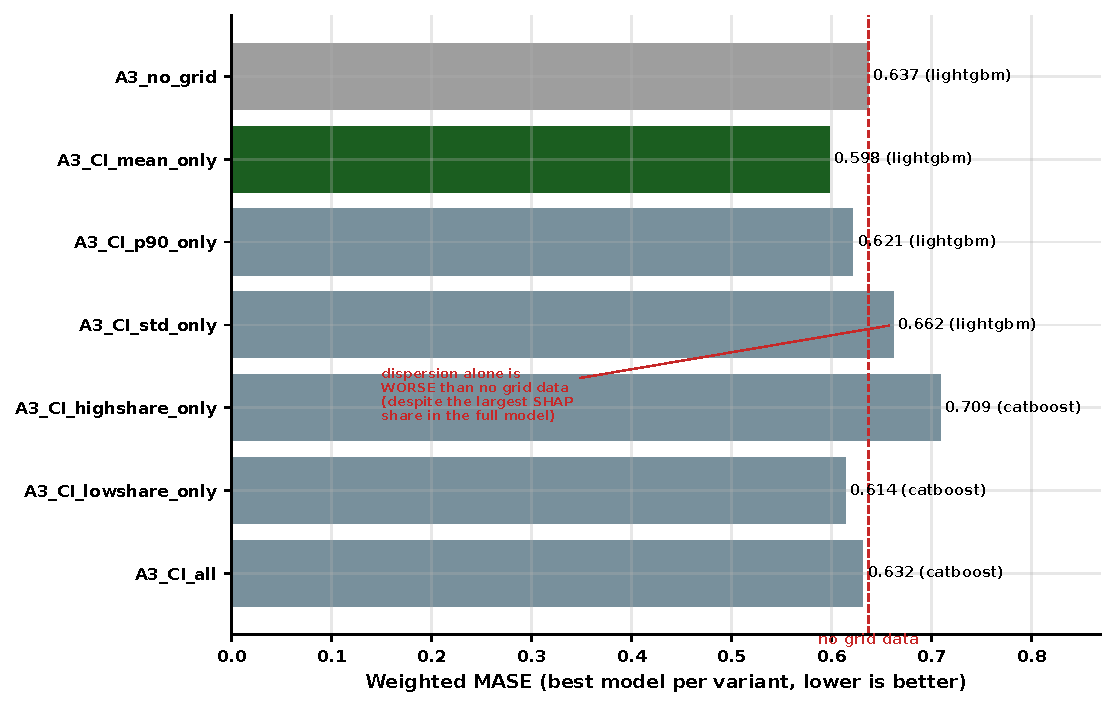
\includegraphics[width=0.85\textwidth]{figures/pdf/main/fig_ci_decomposition.pdf}
\caption{Carbon-intensity statistic decomposition. Weighted MASE for the best model within each single-statistic variant; the dashed line marks the no-grid baseline. Every statistic tested alone except the mean, the low-intensity share, and the 90th percentile falls on or behind that baseline.}
\label{fig:decomposition}
\end{figure}

\subsection{What does grid carbon-intensity dispersion represent?}\label{sec:mechanism}

Section~\ref{sec:decomposition} establishes that dispersion's attribution share is a joint, not standalone, property, but not what dispersion mechanistically tracks. Two candidate explanations are tested against data already available from the retrieved grid record, without new data collection. The first is system-predictability stress: the GB Carbon Intensity API publishes its own half-hourly forecast alongside the outturn value, so the forecast error (outturn minus forecast) is a direct measure of how far the system deviated from the operator's own real-time expectation. The second is renewable intermittency, proxied by the within-quarter standard deviation of the half-hourly wind generation share.

Neither candidate correlates strongly with \texttt{Grid\_CI\_std} over the 28-quarter common period (Figure~\ref{fig:mechanism}a): the mean absolute forecast error correlates at $r=0.03$, the standard deviation of the signed forecast error at $r=0.16$, and wind-share dispersion at $r=0.37$. Tested as a standalone predictor (Figure~\ref{fig:mechanism}b), forecast-error dispersion alone reaches WMASE 0.643 -- close to \texttt{Grid\_CI\_std} alone (0.662) despite the weak correlation between the two, and still behind the mean alone (0.598). \textbf{What \texttt{Grid\_CI\_std} mechanistically represents remains an open question after this test: it is not well explained by either operator forecast-error stress or wind intermittency alone}, and the result should not be over-interpreted as identifying either mechanism. Demand-side volatility and interconnector flow variability are two further candidates that this study's data sources do not cover and that a future extension could test directly.

\begin{figure}[H]
\centering
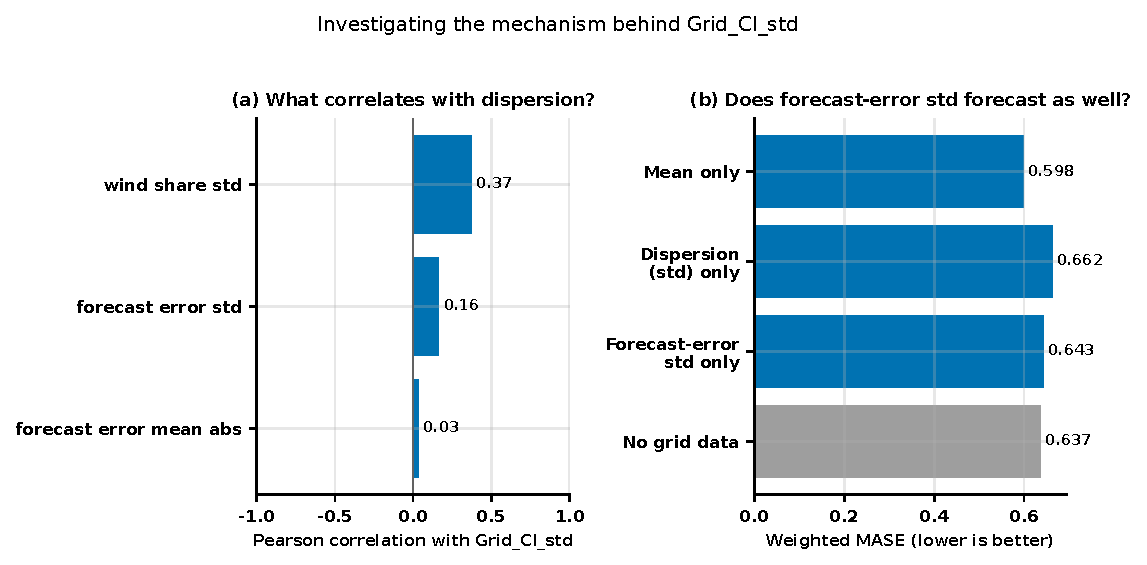
\includegraphics[width=0.85\textwidth]{figures/pdf/main/fig_ci_std_mechanism.pdf}
\caption{Investigating the mechanism behind grid carbon-intensity dispersion. Panel (a): Pearson correlation of two candidate mechanisms with \texttt{Grid\_CI\_std}. Panel (b): weighted MASE when each candidate is tested as a standalone predictor, alongside the mean and dispersion for reference.}
\label{fig:mechanism}
\end{figure}

\subsection{Robustness of the electricity-grid signal}\label{sec:robustness}

The grid advantage remains visible under direct paired testing. Pooling the 27 common horizon-origin comparisons, A3/LightGBM significantly outperforms the engineered-only A2 configuration after Holm--Bonferroni correction ($p=0.031$) and also outperforms the seasonal-naive reference ($p=0.005$). A3 is directionally better than A1 and A4 in 59.3\% of paired origins for each comparison, but these two contrasts do not reach corrected significance at the available sample size. The evidence therefore supports a statistically confirmed advantage over engineered-history-only forecasting and the seasonal benchmark, while the gains over the core baseline and full-fusion alternative remain practically favourable but statistically uncertain (Table~\ref{tab:grid_robustness}).

\begin{table}[p]
\centering
\caption{Robustness of the electricity-grid signal: pooled paired tests and grid-family ablation.}
\label{tab:grid_robustness}
\scriptsize
\begin{threeparttable}
\textit{Panel A: pooled horizon-origin comparisons}\\[2pt]
\begin{tabular}{@{}lrrrrl@{}}
\toprule
Comparison & $n$ & A3 better (\%) & $\Delta$MAE & Holm-adjusted $p$ & Significant \\
\midrule
A3 vs A1 & 27 & 59.3 & $-1933$ & 1.000 & No \\
A3 vs A2 & 27 & 74.1 & $-3216$ & 0.031 & Yes \\
A3 vs A4 & 27 & 59.3 & $-1632$ & 1.000 & No \\
A3 vs seasonal naive & 27 & 74.1 & $-6202$ & 0.005 & Yes \\
\bottomrule
\end{tabular}

\vspace{1.0em}
\textit{Panel B: best model within each grid-ablation variant}\\[2pt]
\begin{adjustbox}{max width=\textwidth}
\begin{tabular}{@{}llrrrrr@{}}
\toprule
Variant & Best model & Features & WMASE & H1 & H2 & H4 \\
\midrule
Full A3 & LightGBM & 23 & \textbf{0.454} & \textbf{0.376} & \textbf{0.575} & \textbf{0.467} \\
No grid information & LightGBM & 11 & 0.637 & 0.801 & 0.542 & 0.369 \\
No carbon-intensity statistics & LightGBM & 18 & 0.664 & 0.623 & 0.690 & 0.728 \\
No generation-mix variables & CatBoost & 18 & 0.627 & 0.697 & 0.560 & 0.554 \\
Carbon-intensity variables only & CatBoost & 16 & 0.589 & 0.661 & 0.478 & 0.576 \\
Generation-mix variables only & CatBoost & 16 & 0.745 & 0.701 & 0.693 & 0.931 \\
\bottomrule
\end{tabular}
\end{adjustbox}
\begin{tablenotes}[flushleft]
\footnotesize
\item Negative $\Delta$MAE favours A3. Holm--Bonferroni-adjusted values are based on pooled Wilcoxon signed-rank tests. Ablation results report the lowest-WMASE model within each variant and therefore form a sensitivity analysis rather than a fixed-model decomposition. The Full A3 row is the same fit reported in Table~\ref{tab:finalists} and Section~\ref{sec:shap}.
\end{tablenotes}
\end{threeparttable}
\end{table}

Table~\ref{tab:dm} and Figure~\ref{fig:per_horizon} extend Panel A with a per-horizon breakdown and the Diebold--Mariano confirmation described in Section~\ref{sec:methodology}. No individual horizon survives Holm correction under the Wilcoxon test for any comparison -- only the pooled result does -- but the Diebold--Mariano test, whose long-run-variance estimator explicitly accounts for the serial correlation expected in $h$-step-ahead errors, finds that \textbf{A3 significantly beats A2 at the one-quarter horizon individually} (DM statistic $-3.63$, Holm-corrected $p=0.037$). This is convergent, not merely repeated, evidence: two tests built on different assumptions agree at H1, and neither is used to inflate a claim the other test does not support. The Diebold--Mariano estimator is undefined at H4 for every comparison, as anticipated in Section~\ref{sec:methodology}: with eight paired origins and a lag truncation of three, the long-run variance estimate is not reliably positive, and the test correctly declines to report a number the sample cannot support rather than returning an unstable one.

\begin{table}[!htbp]
\centering
\caption{Per-horizon significance, including Diebold--Mariano confirmation.}
\label{tab:dm}
\scriptsize
\begin{adjustbox}{max width=\textwidth}
\begin{tabular}{@{}llrrrrrr@{}}
\toprule
Comparison & Horizon & $n$ & A3 better (\%) & Wilcoxon Holm-$p$ & DM statistic & DM Holm-$p$ & DM significant \\
\midrule
A3 vs A1 & H1 & 11 & 72.7 & 0.293 & $-2.42$ & 0.180 & No \\
A3 vs A1 & H2 & 8 & 50.0 & 1.000 & $-2.49$ & 0.180 & No \\
A3 vs A1 & H4 & 8 & 50.0 & 1.000 & -- & -- & Undefined \\
A3 vs A2 & H1 & 11 & 72.7 & 0.191 & $-3.63$ & \textbf{0.037} & \textbf{Yes} \\
A3 vs A2 & H2 & 8 & 62.5 & 1.000 & $-0.67$ & 1.000 & No \\
A3 vs A2 & H4 & 8 & 87.5 & 1.000 & -- & -- & Undefined \\
A3 vs A4 & H1 & 11 & 63.6 & 1.000 & $-1.78$ & 0.318 & No \\
A3 vs A4 & H2 & 8 & 50.0 & 1.000 & $-0.51$ & 1.000 & No \\
A3 vs A4 & H4 & 8 & 62.5 & 1.000 & -- & -- & Undefined \\
A3 vs naive & H1 & 11 & 81.8 & 0.241 & $-2.94$ & 0.103 & No \\
A3 vs naive & H2 & 8 & 75.0 & 0.430 & $-2.92$ & 0.134 & No \\
A3 vs naive & H4 & 8 & 62.5 & 1.000 & -- & -- & Undefined \\
\bottomrule
\end{tabular}
\end{adjustbox}
\end{table}

\begin{figure}[H]
\centering
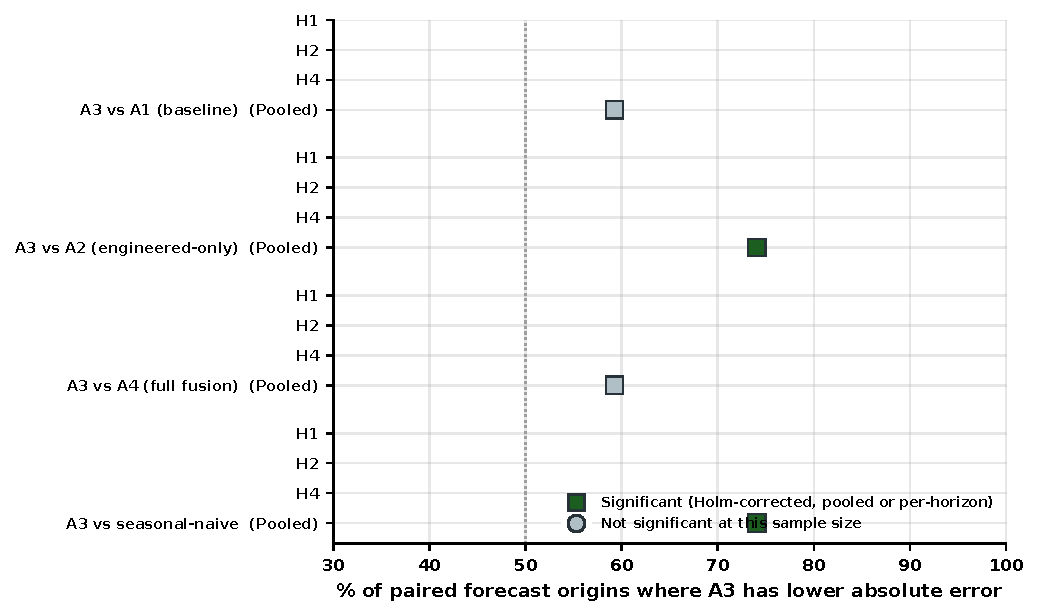
\includegraphics[width=0.85\textwidth]{figures/pdf/main/fig_per_horizon_significance.pdf}
\caption{Per-horizon robustness: share of paired forecast origins where A3 has lower absolute error, by comparison and horizon. Filled markers indicate significance after Holm correction (pooled or per-horizon, either test).}
\label{fig:per_horizon}
\end{figure}

The result is not an artefact of the Google mobility convention. Across four mobility treatments---the primary neutral-zero convention (M0), complete removal of mobility variables (M1), an availability-aware encoding (M2), and a COVID-window-restricted sensitivity design (M3)---A3 ranks first among A1--A4 in every case. Removing mobility narrows the A3--A1 WMASE margin from 0.175 to 0.090, indicating that mobility carries useful information, but it does not reverse the configuration ranking. M3 uses a smaller restricted evaluation sample and is interpreted as a sensitivity check rather than a directly comparable primary estimate (Supplementary Figure S1 and Table S5).

Ablation identifies the source of the grid gain at the family level. The full A3 specification achieves WMASE 0.454, compared with 0.589 for carbon-intensity variables only, 0.627 when generation-mix variables are removed, 0.637 with all grid information removed, 0.664 when carbon-intensity variables are removed, and 0.745 for generation-mix variables only (Figure~\ref{fig:grid_ablation} and Table~\ref{tab:grid_robustness}). Carbon-intensity distributional statistics therefore carry the main predictive signal at the family level, consistent with the within-family decomposition in Section~\ref{sec:decomposition}. Generation-mix shares alone do not improve the baseline at this sample size, although the full A3 combination remains better than either information family in isolation, indicating complementary rather than redundant information.

\begin{figure}[H]
\centering

\includegraphics[width=0.85\textwidth]{figures/pdf/main/fig_grid_ablation.pdf}
\caption{Grid-signal ablation. Weighted MASE is shown for the best-performing model within each information variant. Lower values are better; the complete A3 information block remains the leading specification.}
\label{fig:grid_ablation}
\end{figure}

Origin-level diagnostics further show that the aggregate improvement is not driven by one exceptional quarter. The champion beats the seasonal-naive error in 20 of 27 horizon-origin combinations, with gains distributed across 2022Q3--2025Q1. The largest exceptions are concentrated mainly at the four-quarter horizon in 2024. This pattern supports the interpretation of the grid contribution as a recurring near-term signal rather than a single-shock artefact (Supplementary Figure S2 and Table S6).

\subsection{Empirical prediction intervals}\label{sec:intervals}

The results above report point forecasts. An operational monitoring use, discussed in Section~\ref{sec:discussion}, requires a range around that point. With only 8--11 forecasts per horizon, a distributional assumption or a quantile-regression model would overstate what this sample size can support; instead, a leave-one-out empirical quantile interval is constructed at each horizon, so that no observation ever informs its own interval, and its coverage is checked honestly rather than assumed.

Table~\ref{tab:intervals} reports the result plainly: nominal 80\% intervals achieve only 62--64\% empirical leave-one-out coverage across all three horizons, and nominal 50\% intervals achieve 25--50\%. \textbf{The intervals as constructed are anti-conservative -- narrower than their stated level -- at this sample size.} This is itself an expected consequence of estimating tail quantiles from 8--11 points, and it is reported as a property of the method at this sample size rather than adjusted away by widening the intervals until they pass their own calibration check. Figure~\ref{fig:intervals} plots the resulting fan charts against the champion's actual out-of-sample trajectory. Any use of these intervals for monitoring should treat them as an indicative range, not a validated confidence level.

\begin{table}[!htbp]
\centering
\caption{Empirical leave-one-out interval calibration.}
\label{tab:intervals}
\begin{tabular}{@{}llrrr@{}}
\toprule
Horizon & Nominal level & $n$ & Empirical coverage & Mean half-width (kt CO$_2$e) \\
\midrule
H1 & 50\% & 11 & 36.4\% & 1234 \\
H1 & 80\% & 11 & 63.6\% & 3205 \\
H2 & 50\% & 8 & 50.0\% & 1974 \\
H2 & 80\% & 8 & 62.5\% & 5465 \\
H4 & 50\% & 8 & 25.0\% & 2335 \\
H4 & 80\% & 8 & 62.5\% & 4210 \\
\bottomrule
\end{tabular}
\end{table}

\begin{figure}[p]
\centering
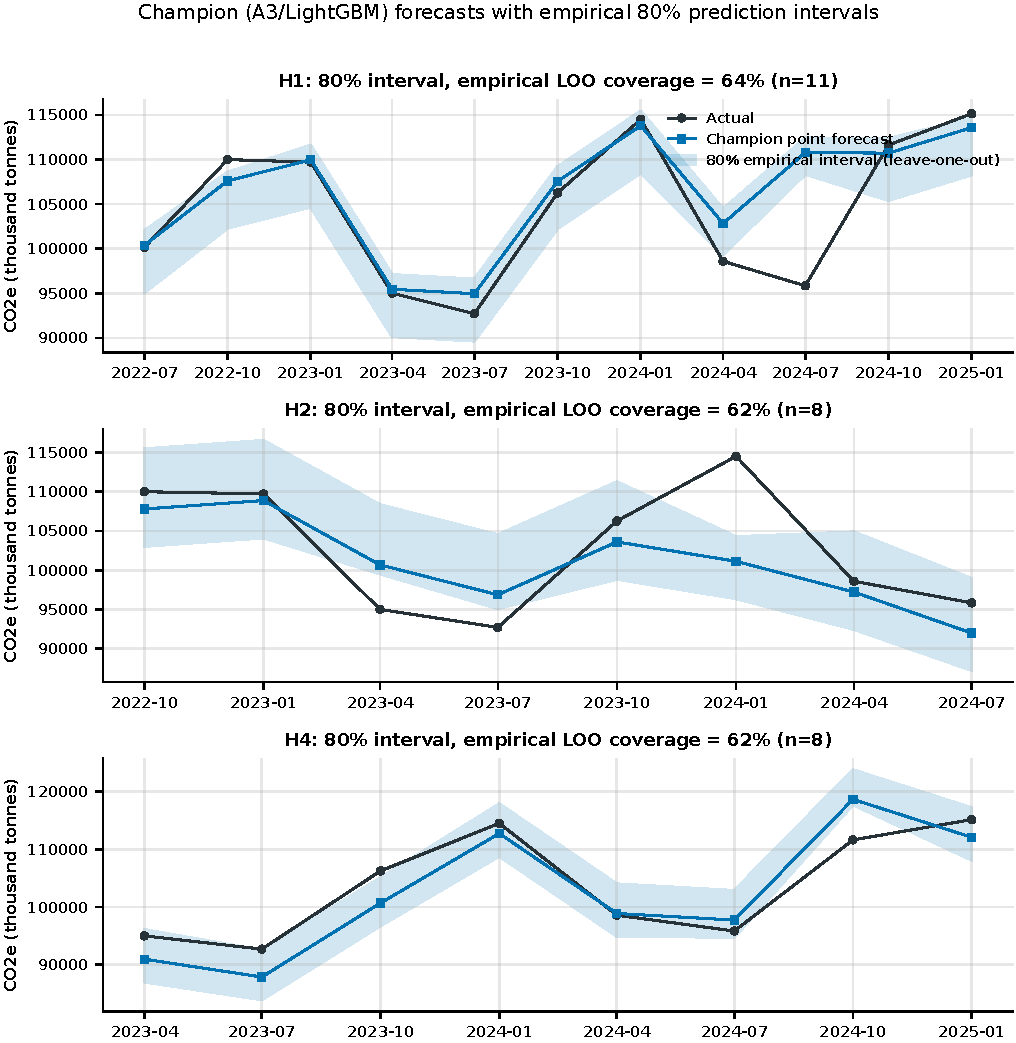
\includegraphics[width=0.8\textwidth,height=0.8\textheight,keepaspectratio]{figures/pdf/main/fig_champion_prediction_intervals.pdf}
\caption{Champion forecasts with empirical 80\% leave-one-out prediction intervals at each horizon, plotted against the actual out-of-sample trajectory. Panel titles report the empirical coverage achieved.}
\label{fig:intervals}
\end{figure}

\subsection{A live demonstration of the deployed model}\label{sec:nowcast}

Every result so far is a backtest: a forecast is scored only once its target quarter is already known. To demonstrate the framework as an operational instrument rather than a retrospective exercise, the champion's direct H1, H2 and H4 models are re-fitted on all available common-period history and applied at the true current forecast origin -- 2025Q1, the most recent quarter with a published target. Because the framework forecasts directly from a known origin to a future target ($X_t\rightarrow y_{t+h}$), this uses exclusively real, already-observed inputs: no future-quarter covariate is synthesised, unlike a recursive multi-step scheme that would need one.

Table~\ref{tab:nowcast} reports the resulting forecasts for 2025Q2, 2025Q3 and 2026Q1. These are demonstrations of the deployed mechanism, not scored accuracy results: no published target yet exists for these quarters, and the numbers should not be cited as a validated forecast-error claim. A separate, concrete observation supports the framework's timeliness argument directly: the NESO Carbon Intensity API already contains real grid data for five quarters beyond the current target origin (through 2026Q2, Table~\ref{tab:source_quality}), while the macroeconomic and mobility series this framework also depends on are bounded by their own release schedules. The grid predictor for the next forecast origin is therefore already available before the wider information set catches up -- direct evidence for, rather than an assertion of, the early-warning framing developed in Section~\ref{sec:policy}.

\begin{table}[!htbp]
\centering
\caption{Live nowcast from the current data origin (2025Q1). Demonstration of the deployed mechanism; not a scored accuracy result.}
\label{tab:nowcast}
\begin{tabular}{@{}lllrr@{}}
\toprule
Origin & Horizon & Target quarter & Point forecast (kt CO$_2$e) & Training pairs \\
\midrule
2025Q1 & H1 & 2025Q2 & 97{,}739 & 27 \\
2025Q1 & H2 & 2025Q3 & 97{,}823 & 26 \\
2025Q1 & H4 & 2026Q1 & 112{,}784 & 24 \\
\bottomrule
\end{tabular}
\end{table}

\section{Discussion}\label{sec:discussion}

\subsection{The story is about information, not simply complexity}

The experiment began with the expectation that a carefully engineered or selected feature set might improve a short emissions series by concentrating signal. The final evidence is more specific, and more qualified than a single SHAP ranking alone would suggest. The best unrestricted and overall model is not the largest pool and does not use feature selection; it combines the baseline variables with high-frequency electricity-grid information. Adding all engineered variables weakens that advantage, while the compact Stream-B finalist trades some accuracy for parsimony and stability.

The family-level ablation and the within-family decomposition together sharpen the mechanism behind this finding, and they must be read as a pair rather than separately. At the family level, carbon-intensity statistics are the principal source of the grid contribution: carbon-intensity-only forecasting improves on removing grid information altogether, whereas generation-mix-only information performs worse than the no-grid baseline, and the complete A3 specification remains best, showing that generation-mix and transition indicators complement the dominant carbon-intensity signal even when they are not sufficient on their own. Within the carbon-intensity family, however, the decomposition in Section~\ref{sec:decomposition} shows that dispersion's large attribution share is not evidence that dispersion is the best carbon-intensity statistic in isolation -- tested alone, the mean is. \textbf{The two findings are consistent, not contradictory: SHAP attribution reports a feature's marginal contribution given the rest of the model, and dispersion earns its share by adding information on top of the mean and upper tail once they are already present, not by being individually superior to them.} The corollary is practical rather than semantic: no single carbon-intensity statistic, however large its attribution share, can substitute for the full grid feature set without a material cost in accuracy.

Model architecture and predictor governance still matter. LightGBM wins the final comparison, CatBoost remains strong across many candidate cells, and LSTM is poorly matched to the short common panel. Governance remains essential for preventing target leakage and enforcing release timing. However, once those controls are imposed, the largest practical gain comes from adding the right external process, in its complete distributional form, rather than from expanding or aggressively reducing the predictor set, or from reading a single leading SHAP value as a standalone recommendation.

\subsection{Feature selection is a choice about priorities}

Feature selection does not fail uniformly. B3 wrapper LightGBM preserves most of the A3 signal with 15 rather than 23 variables and achieves the best four-quarter family result, MASE 0.356. If the objective were to reduce dimensionality while retaining grid information, this would be a persuasive alternative. Equal-weight VIKOR instead selects a six-variable B1 CatBoost model because it is smaller and less variable across folds. The difference demonstrates why feature selection should not be judged only by whether it lowers the minimum error. It changes the shape of the decision problem.

The selector results also warn against treating consensus as automatically robust. When all 37 variables enter B4, agreement fragments and no feature receives three votes. Permutation stability performs poorly across nearly all settings because it repeatedly selects a narrow mobility-heavy set. Wrapper selection has the best mean accuracy but high rank dispersion. The appropriate selector therefore depends on the pool and the intended trade-off. A method that performs well in B3 need not remain reliable in B4.

\subsection{Implications for quarterly transition monitoring}\label{sec:monitoring}

For policy monitoring, the one-quarter result remains the most operationally relevant: H1 MASE is 0.3763, about 62\% below the seasonal-naive scale. The advantage is not confined to a single shock period. The champion beats the seasonal-naive error in 20 of 27 horizon-origin comparisons, and SHAP shows that grid-family predictors account for more than 60\% of total attribution in pre-COVID, COVID and post-COVID regimes. This combination of forecast and attribution stability, together with the live demonstration in Section~\ref{sec:nowcast}, supports treating grid dynamics as a recurring near-term signal that a monitoring system can act on as it is published, rather than a pandemic-specific artefact or a purely retrospective finding.

The framework should therefore be viewed as an early-warning layer rather than a substitute for the official inventory. A quarterly model can flag divergence from an expected emissions path, indicate when electricity-system operating conditions are carrying unusual predictive information and support faster diagnosis of whether a national trajectory is changing. It cannot identify the causal effect of renewable deployment, separate sector-specific contributions or replace reconciled inventory accounting. Those tasks require structural, sectoral or causal designs. The practical implication for sustainable-energy monitoring is that high-frequency operational data can add value when they are aggregated with explicit semantics and temporal governance. The ablation and decomposition results together suggest that the most useful signal is not simply the reported renewable share, nor any single carbon-intensity statistic, but the joint distribution of grid carbon intensity within a quarter, deployed as a whole. Monitoring systems that retain this operating variability may therefore detect national carbon changes earlier than systems based only on annual transition indicators or engineered historical emissions features.

\subsection{Policy and economic implications}\label{sec:policy}

The family-level and within-family results in Sections~\ref{sec:decomposition} and~\ref{sec:robustness} support a specific reframing that the SHAP ranking alone does not. Generation-mix shares -- renewable, low-carbon, fossil, gas and wind -- are the variables most directly tied to \emph{capacity}: how much low-carbon generation has been built. Carbon-intensity dispersion, by contrast, is closer to a measure of \emph{operational flexibility}: how often the system is forced to fall back on carbon-intensive generation to balance supply and demand within a quarter. The finding that carbon-intensity statistics as a family (WMASE 0.589) outperform generation-mix shares as a family (0.745) -- which in turn underperforms dropping grid information entirely (0.637) -- is therefore not only a modelling result. It suggests that, at a quarterly forecasting resolution, the pace at which flexibility and storage are deployed carries more forecast-relevant information than the pace at which capacity is added. Consistent with Section~\ref{sec:mechanism}, this is a predictive association, not a causal or mechanistic claim: what specifically drives carbon-intensity dispersion remains an open question. It nonetheless reframes what a monitoring system built on this signal should track, and for whom.

That reframing maps onto concrete institutional use, summarised in Figure~\ref{fig:policy_map}. For a system operator and regulator (in the UK context, NESO and Ofgem), a rising quarterly carbon-intensity dispersion is an early, model-agnostic indicator that flexibility and storage procurement may be lagging the pace of intermittent generation growth -- a signal available from settlement-period data well before it would be visible in annual capacity statistics. For climate policy delivery bodies (DESNZ, the Climate Change Committee), the H1 nowcast (MASE 0.376, a 62\% reduction in scaled error relative to the seasonal-naive benchmark, demonstrated live in Section~\ref{sec:nowcast}) offers an in-year complement to the reconciled annual inventory: a divergence flag that could prompt review ahead of a Carbon Budget Delivery Plan progress report, without replacing the inventory itself. For energy investors and carbon-market participants, the finding that average generation-mix disclosures alone are a weaker predictive signal than intensity variability is a caution against relying on capacity-only transition-risk screens. For fiscal and statistical bodies (HM Treasury/OBR, the Office for National Statistics), a transparent, leakage-audited nowcast, together with the prediction intervals in Section~\ref{sec:intervals}, is best positioned as a faster-turnaround cross-check alongside existing in-year forecasting work, not a substitute for the official experimental quarterly estimate.

\begin{figure}[H]
\centering
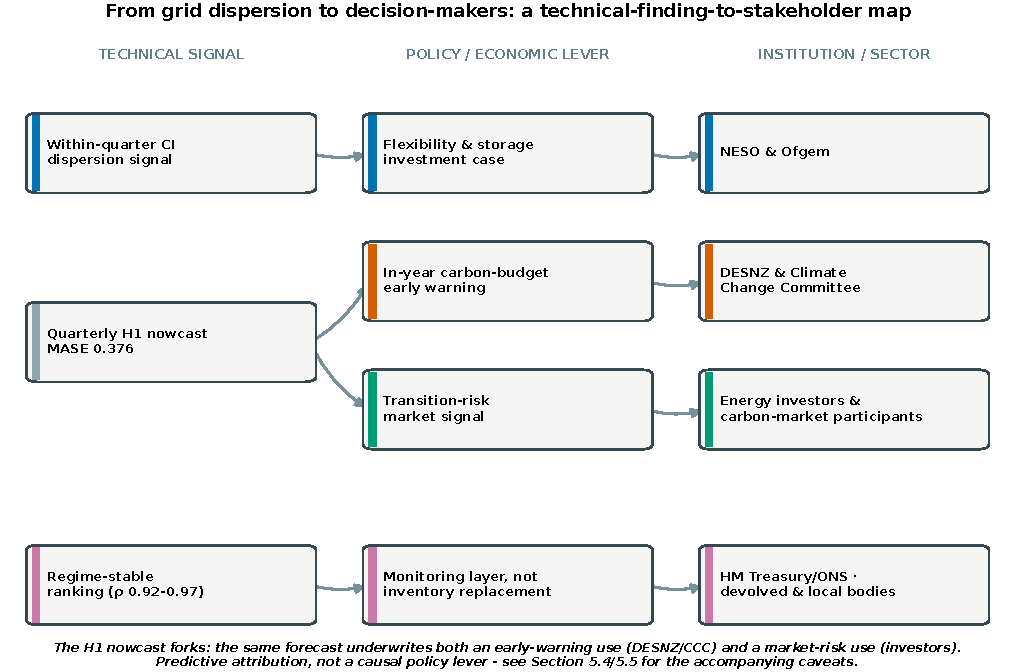
\includegraphics[width=0.85\textwidth]{figures/pdf/main/fig_policy_stakeholder_map.pdf}
\caption{From grid dispersion to decision-makers: a technical-finding-to-stakeholder map. The H1 nowcast forks -- the same forecast underwrites both an early-warning use and a market-risk use. Predictive attribution, not a causal policy lever.}
\label{fig:policy_map}
\end{figure}

These are monitoring, not compliance, use cases, and they inherit the limitations set out in Section~\ref{sec:limitations}: a 28-quarter common evaluation window, regime subsamples as small as seven observations, prediction intervals that are indicative rather than calibrated, and predictive attribution that should not be read as identifying which intervention would reduce emissions fastest. Within those limits, the operational-flexibility framing gives the electricity-grid signal a concrete institutional audience that a single-statistic reading of the SHAP ranking does not.

\subsection{Limitations and next steps}\label{sec:limitations}

The common-period sample remains the main limitation. Grid availability restricts the primary comparison to 2018 onward, leaving 11 H1 forecasts and eight H2/H4 forecasts, or 27 paired horizon-origin observations when pooled. This is sufficient to identify a significant advantage of A3 over A2 and the seasonal-naive benchmark after Holm--Bonferroni correction, under both the Wilcoxon and, at H1, the Diebold--Mariano test, but not to establish corrected significance against A1 or A4. The latter comparisons should therefore be interpreted as directionally favourable rather than conclusive. The Diebold--Mariano test is itself undefined at H4 given this sample size, for the reason set out in Section~\ref{sec:methodology}.

The earlier concern about the Google mobility zero convention is reduced by the sensitivity analysis in Section~\ref{sec:robustness}. A3 remains the leading configuration when mobility is removed, encoded with an availability indicator, or evaluated in a restricted COVID-window design. Nevertheless, the mobility archive still ends in October 2022 and cannot serve as a permanent operational series. M3 also uses a smaller restricted sample, so it is informative about ranking robustness rather than directly comparable absolute WMASE.

Interpretability carries three specific boundaries. First, SHAP describes predictive attribution and does not identify causal effects. Second, while Section~\ref{sec:decomposition} isolates each carbon-intensity statistic's standalone contribution, Section~\ref{sec:mechanism} shows that what dispersion mechanistically represents is still an open question: two plausible candidates, operator forecast-error stress and wind intermittency, do not explain it, and demand-side or interconnector volatility remain untested. Third, the empirical prediction intervals in Section~\ref{sec:intervals} are anti-conservative at this sample size and should be read as indicative, not calibrated.

Finally, the framework should be replicated across countries and sectors. Electricity systems differ in generation mix, interconnection, market design and the relationship between grid emissions and economy-wide \coo{}. Cross-country replication is needed to determine whether the dominance of grid carbon-intensity information over generation-mix shares is a general transition signal or a feature of the UK period studied here; the leakage-audited registry design and the within-family decomposition method are directly transferable to that test even where the UK-specific ranking of individual statistics may not be. Sectoral targets could reveal which parts of the economy transmit the grid signal into national emissions.

\section{Conclusions}\label{sec:conclusion}

Quarterly emissions forecasting becomes more useful when it is treated as an information-governance problem rather than a contest between algorithms. \qdecem{} compares four predictor pools with and without five feature-selection strategies while keeping feature construction, selection, optimisation and evaluation inside nested temporal boundaries.

On the common UK panel, A3/LightGBM is the overall champion, achieving WMASE 0.4541 with H1, H2 and H4 MASE of 0.3763, 0.5751 and 0.4672. TreeSHAP analysis shows that \texttt{Grid\_CI\_std} carries the largest single share of predictive attribution, 31.8\%, followed by \texttt{Grid\_CI\_mean} and \texttt{Grid\_CI\_p90}, with grid-family predictors retaining 61.1--69.0\% of attribution across pre-COVID, COVID and post-COVID regimes; the hierarchy is stable across regimes rather than being driven by the pandemic period. A within-family decomposition qualifies that ranking precisely: tested alone, the mean outperforms dispersion, and dispersion alone underperforms a no-grid baseline, so dispersion's attribution share is a joint property of the full carbon-intensity distribution rather than evidence that it is individually the strongest statistic. What dispersion mechanistically represents remains open after testing two candidate explanations.

Robustness checks support the configuration-level conclusion from several directions. A3 remains the leading configuration under all four mobility treatments; it significantly outperforms the engineered-only A2 configuration and the seasonal-naive benchmark after Holm--Bonferroni correction, confirmed at the one-quarter horizon individually by a Diebold--Mariano test; and origin-level gains are distributed across most of the evaluation window rather than concentrated in one quarter. Family-level ablation shows that carbon-intensity distributional statistics, rather than generation-mix shares alone, provide the main grid contribution, although the complete A3 information block performs best overall. A live demonstration from the true current data origin, together with empirical prediction intervals, extends the framework toward an operational monitoring instrument rather than a purely retrospective exercise, while making explicit where that instrument's uncertainty is currently under-characterised.

These findings remain conditional on a short UK evaluation window and should not be interpreted as causal evidence or a universal model ranking. Within those limits, the study provides consistent evidence that timely electricity-system operating information -- specifically the joint distribution of grid carbon intensity, not any single statistic within it -- can improve near-term national emissions monitoring more than simply enlarging or automatically reducing a conventional predictor set.

\section*{CRediT authorship contribution statement}
\textbf{Mohsen Asghari Ilani:} Conceptualization, Methodology, Software, Formal analysis, Data curation, Writing--original draft, Writing--review \& editing. \textbf{Hamidreza Eskandari:} Methodology, Validation, Writing--review \& editing, Supervision. \textbf{Mike Banad:} Validation, Writing--review \& editing.

\section*{Data and code availability}
The manuscript is based on the audited result tables and figure manifest supplied with the \texttt{qdecem} software package, archived at \url{https://doi.org/10.5281/zenodo.22820748} (version-specific release) and developed at \url{https://github.com/Mohsena1990/co2_emission_prediction}.

\section*{Declaration of competing interest}
The authors declare no known competing financial interests or personal relationships that could have appeared to influence the work reported in this paper.

% \section*{Acknowledgements}
% Insert funding, supervisory, institutional, and data-provider acknowledgements here.

\clearpage
\bibliographystyle{elsarticle-num-names}
\bibliography{references}

\end{document}
